% Laborationsmall.tex
\documentclass[a4paper]{article}

\usepackage[swedish]{babel}
\usepackage[utf8x]{inputenc}

\usepackage{multicol}
\usepackage[vmargin=3cm,hmargin=2cm]{geometry}
\usepackage{parskip}
\usepackage[runin]{abstract}
\renewcommand{\abstitleskip}{0mm}

\usepackage{hyperref}
\usepackage{amsmath}
\usepackage{lmodern}
\usepackage[T1]{fontenc}
\usepackage{pgfplots}
\usetikzlibrary{decorations.pathreplacing}
\usetikzlibrary{arrows.meta}

\addto\extrasswedish{%
	\def\equationautorefname{Ekvation}%
	\def\figureautorefname{Figur}%
	\def\tableautorefname{Tabell}%
	\def\sectionautorefname{Rubrik}%
	\def\subsectionautorefname{Underrubrik}%
	\def\pageautorefname{Sida}%
}

\usepackage{graphicx}
\usepackage{ccaption}
\captionnamefont{\it}
\captiontitlefont{\it}

% Hack för att få komma istället för punkt i matematiska uttryck
% $3.141592$ blir 3,141592
% Om man använder komma direkt får man ett litet oönskat mellanrum:
% $3,141592$ blir 3, 141592
\DeclareMathSymbol{,}{\mathpunct}{letters}{"3B}
\DeclareMathSymbol{.}{\mathord}{letters}{"3B}
\DeclareMathSymbol{\decimal}{\mathord}{letters}{"3A}

% Kommando för att få icke-kursiva enheter i matematiska uttryck
% $10\unit{km}$ blir 10 km
\newcommand{\unit}[1]{\ensuremath{\,\mathrm{#1}}}

\usepackage{lastpage}
\usepackage{fancyhdr}
\pagestyle{fancy}
\fancyhf[C]{\thepage}
\fancyhead[C]{Våglära och optik, FAFF30}
\fancyhead[R,L]{}
\fancypagestyle{plain}{
  \fancyhead{}
}
\setcounter{secnumdepth}{-1}

\title{Laborationen ”Polarisation”}
\author{Johan Mauritsson\\Lunds Universitet}

\makeatletter
\renewcommand{\section}{\@startsection
{section}%                   % the name
{1}%                         % the level
{0mm}%                       % the indent
{-\baselineskip}%            % the before skip
{0.5mm}%          % the after skip
{\normalfont\bfseries}} % the style
%\renewcommand{\sectionmark}[1]{ }
%\renewcommand{\thesection}{}

\renewcommand*\maketitle{
  {
    \begin{center}
      {\huge\bfseries \@title}\\
      \vspace{5mm}
      {\large \@author}
    \end{center}
    \vspace{2mm}
  }
}
\makeatother

\begin{document}
\maketitle


\begin{abstract}
  Kort beskrivning  av resultaten (5-10  rader). Det ska inte  vara en
  innehållsbeskrivning (först gör vi det, sen använder vi den metoden,
  och så jämför vi det med de där tidigare kända resultaten, etc) utan
  vara   koncentrerat  till   ”resultatet”,   vad   man  kommer   fram
  till. Sammanfattningen är uppsatsens löpsedel. Den ska vara kort och
  kärnfull och locka läsare genom att  effektivt göra klart vad det är
  man uppnår genom att läsa rapporten.
\end{abstract}

\vspace{2mm}

\hspace{-3mm}
\begin{tabular}{ll}
Laborationen genomförd: &	2017-03-27 \\
Rapporten kamratgranskad: &	2013-xx-xx \\
Lämnad till handledare: &	2013-xx-xx \\
\end{tabular}

\vspace{3mm}

\begin{multicols}{2}
  \section*{Inledning}
  %Preliminär beskrivning av uppgiften  i lättfattliga termer. Bakgrunden till att man intresserar sig för detta problem, denna uppgift. Hur den ingår i ett större sammanhang.

%  En detaljerad beskrivning av vad det hela går ut på, och vad exakt din uppgift   i    sammanhanget   är.    Utrustningsförutsättningar.   Det
%  ursprungligen avsedda målet. Även den i ämnet oinsatte ska ha en ärlig
%  chans att förstå de stora dragen.
%
%  Beskrivning av hur rapporten är uppbyggd, för att göra det möjligt för
%  läsaren att förstå vad som  pågår, ge läsaren rätta förväntningar, och
%  för  att  underlätta direktåtkomst  av  för  den individuelle  läsaren
%  särskilt intressanta delar.

  \section{Teori}
  
  För att räkna ut avlänkningsvinkeln i ett prisma ritas \autoref{fig:prisma} upp med hjälpvinklarna $\alpha'$, $\beta'$ och $\beta$. Med hjälp av vinkelsumman i triangeln som bildas av prismat samt strålen genom prismat fås
  
  \begin{equation} \label{eq:triSum}
  	(90° - \alpha') + (90° - \beta') + A = 180°.
  \end{equation}
  
  Med denna ekvation tillsammans med Snells lag kan följande ekvationer härledas

  \begin{align} 
  \label{eq:alphaPrim}
  \alpha' &= \arcsin\left(\frac{\sin\alpha}{n}\right)\\
  \label{eq:beta}
  \beta &= \arcsin\left(n \sin\beta'\right)\\
  \label{eq:betaPrim}
  \beta' &= A-\alpha'\\
  \label{eq:delta}
  \delta &= \alpha+\beta-\alpha'-\beta'
  \end{align}
  
  som kan kombineras till

  \begin{equation} \label{eq:avlänkning}
  \delta = \alpha-A+\arcsin\left(n \sin\left(A-\arcsin\left(\frac{\sin\alpha}{n}\right)\right)\right).
  \end{equation}

  \section{Metod}
  % De  olika  stegen  i  uppgiftens genomförande.  Till  exempel  val  av
  % algoritmer,  programspråk och  annan programvara,  undersökningsmetod,
  % statistiska  metoder. Där  valmöjligheter finns,  diskutera de  gjorda
  % valen.
  
  % Beskrivning av mätning av fokallängd här.
  
  En laser leddes genom ett optiskt fiber och en lins användes för att kollimera stålen när den lämnade fibret. Två irisar placerades på en väldefinierad linje och lasern leddes genom dessa för att bekräfta att lasern var rak och kollimerad.
  
  Ett prisma på en graderad roterbar platta placerades i laserstrålens väg och en millimetergraderad skärm placerades ut parallell med laserstrålen så att den brutna strålen träffade skärmen enligt \autoref{fig:exp}. Prismat roterades så att laserstrålen träffade rakt på ($\alpha=0$) och prismats rotation antecknades. Sedan roterades prismat 2\textdegree upprepade gånger och positionen där laserstrålen träffade skärmen antecknades och räknades om till vinkeln $\gamma$.
  
  Mätvärdena matades in i matlab och där användes appen ``Curve Fitting'' för att hitta ett brytningsindex så att ekvationen \eqref{eq:avlänkning} gäller så väl som möjligt.

  \section{Resultat}
  %Vad man  kommer fram till?  Om uppgiften innebär programmering  så kan
  %det färdiga programmet i sig vara resultatet.  Här är det i så fall på
  %sin  plats  med  beskrivningar  av programmet,  till  exempel  teknisk
  %beskrivning,    funktionell    beskrivning,    användningsbeskrivning,
  %användargränssnitt  etc.  Genomförandebeskrivning  kommer  i  så  fall
  %närmast att handla om programutvecklingen.

  %Men det kan också vara så  att det snarare är programmets beteende som
  %är resultatet.  Man utvecklar till  exempel en numerisk metod  för att
  %lösa ett problem,  och sedan gör man experiment  med testkörningar och
  %analyserar dessa test.

  \section{Diskussion}
  %Är resultaten rimliga? Vad hade kunnat göras annorlunda?

  \section{Slutsats/avslutning}
  %En   sammanfattning  där   man  till   skillnad  från   den  inledande
  %sammanfattningen förutsätter  att läsaren har läst  rapporten, samt de
  %slutsatser man kan dra av det gjorda arbetet.

  \section{Referenser}
  %Den använda litteraturen.

  \section{Appendix}
  %Eventuell     användarhandledning,     källkod,    anvisningar     för
  %systemgenerering, och liknande som inte  är av omedelbart intresse för
  %den ordinäre läsaren, läggs lämpligen som appendix.

\end{multicols}

\begin{figure}[h]
	\centering
	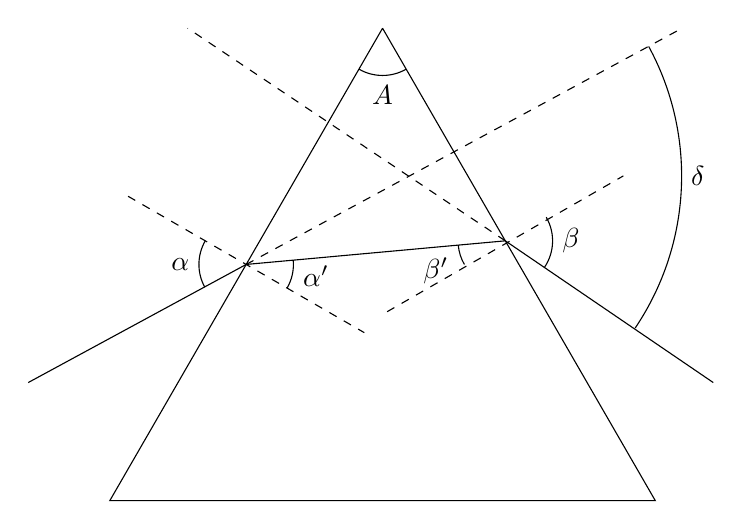
\begin{tikzpicture}[scale=1.5]
		\draw (0, 0) -- ({4/sqrt(3)}, -4) -- ({-4/sqrt(3)}, -4) -- (0, 0); % Triangeln
		
		\draw (-3, -3) -- ({-2/sqrt(3)}, -2) -- ({1.8/sqrt(3)}, -1.8) -- (2.8, -3); % Den brutna ljusstrålen
		\draw [dashed] ({-2/sqrt(3)}, -2) -- ({6 - 2*sqrt(3)}, 0); % Hjälplinjer
		\draw [dashed] ({1.8/sqrt(3)}, -1.8) -- (-1.65, 0);
		\draw [dashed] ({-2/sqrt(3)-1}, {-(6-sqrt(3))/3}) -- ({-2/sqrt(3)+1}, {-(6+sqrt(3))/3});
		\draw [dashed] ({1.8/sqrt(3)-1}, -2.4) -- ({1.8/sqrt(3)+1}, -1.25);
		
		\draw ({-0.4/2}, {-0.4*sqrt(3)/2}) arc [radius=0.4, start angle=240, end angle=300]; % Toppvinkeln
		\draw ({-2/sqrt(3) - (sqrt(3)*0.4)/2}, {-2 + 0.4/2}) arc [radius=0.4, start angle=150, end angle={150+58.45}]; % Infallsvinkeln
		\draw ({0.23 + 2.3*0.83}, {-1.25 - 2.3*0.56}) arc [radius=2.3, start angle=-34, end angle=28.5]; % Avlänkningsvinkeln
		\draw ({1.8/sqrt(3) + 0.4*0.83}, {-1.8 - 0.4*0.56}) arc [radius=0.4, start angle=-34, end angle=30]; % Lämningsvinkeln
		\draw ({-2/sqrt(3) + 0.4*sqrt(3)/2}, {-2 - 0.4*0.5}) arc [radius=0.4, start angle=-30, end angle=5.2]; % Hjälpvinklar
		\draw ({1.8/sqrt(3) - 0.4*0.996}, {-1.8 - 0.4*0.091}) arc [radius=0.4, start angle=185.2, end angle=210];
		%\draw ({-0.21 + 0.2*sqrt(3)/2}, {-2.55 + 0.2*0.5}) arc [radius=0.2, start angle=30, end angle=150];
		
		\node [left] at ({-2/sqrt(3)-0.4}, -2) {$\alpha$};
		\node [right] at ({-2/sqrt(3)+0.4}, -2.1) {$\alpha'$};
		\node [left] at ({1.8/sqrt(3)-0.4}, -2.05) {$\beta'$};
		\node [right] at ({1.8/sqrt(3)+0.4}, -1.8) {$\beta$};
		\node [right] at ({0.23 + 2.3}, -1.25) {$\delta$};
		\node [below] at (0, -0.4) {$A$};
		%\node [above] at (-0.21, -2.35) {$B$};
	\end{tikzpicture}
	\caption{Ljusstråle som bryts genom ett prisma med de hjälpvinklar som behövs för att räkna ut avlänkningsvinkeln.}
	\label{fig:prisma}
\end{figure}
\begin{figure}[h]
	\centering
	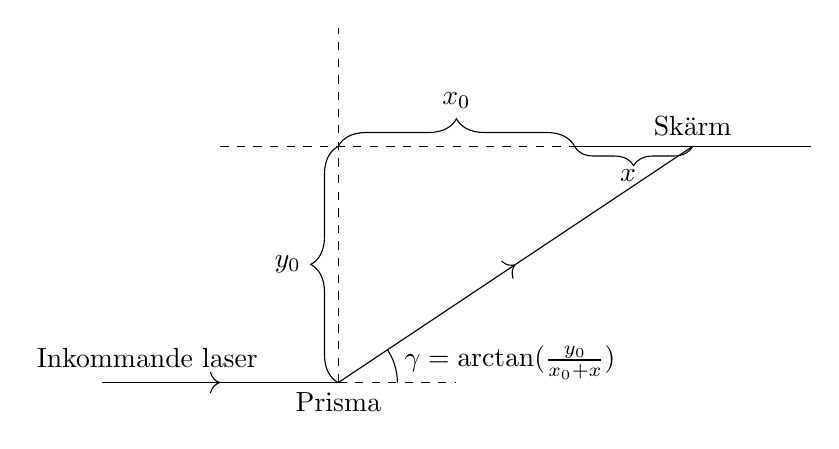
\begin{tikzpicture}[scale=1.5]
		\draw [decorate,decoration={brace,amplitude=10pt}] (0, 0) -- (0, 2) node [midway,left,xshift=-10pt] {$y_0$};
		\draw [decorate,decoration={brace,amplitude=10pt}] (0, 2) -- (2, 2) node [midway,above,yshift=10pt] {$x_0$};
		\draw [decorate,decoration={brace,amplitude=7pt,mirror}] (2, 2) -- (3, 2) node [midway,below,yshift=-5pt,xshift=-2pt] {$x$};
		\draw [dashed] (0, 0) -- (0, 3);
		\draw [dashed] (-1, 2) -- (2, 2);
		\draw (2, 2) -- (4, 2);
		\draw [-{>[scale=1.5]}] (0, 0) -- (1.5, 1);
		\draw (1.5, 1) -- (3, 2);
		\node [below] at (0, 0) {Prisma};
		\node [above] at (3, 2) {Skärm};
		\draw (0.5, 0) arc [radius=0.5, start angle=0, end angle={atan(2/3)}] node [midway,right,yshift=1pt] {$\gamma=\arctan(\frac{y_0}{x_0+x})$};
		\draw [-{>[scale=1.5]}] (-2, 0) -- (-1, 0) node [midway,above,xshift=-5pt,yshift=2pt] {Inkommande laser};
		\draw (-1, 0) -- (0, 0);
		\draw [dashed] (0, 0) -- (1, 0);
	\end{tikzpicture}
	\caption{Experimentuppställning}
	\label{fig:exp}
\end{figure}
\begin{figure}[h]
	\centering
	% This file was created by matlab2tikz.
%
%The latest updates can be retrieved from
%  http://www.mathworks.com/matlabcentral/fileexchange/22022-matlab2tikz-matlab2tikz
%where you can also make suggestions and rate matlab2tikz.
%
\definecolor{mycolor1}{rgb}{0.07059,0.40784,0.70196}%
%
\begin{tikzpicture}

\begin{axis}[%
width=0.951\textwidth,
height=0.438\textwidth,
at={(0\textwidth,0\textwidth)},
scale only axis,
xmin=38.2,
xmax=77.8,
xlabel style={font=\color{white!15!black}},
xlabel={infallsvinkel (°)},
ymin=46.059,
ymax=54.402,
ylabel style={font=\color{white!15!black}},
ylabel={avlänkning (°)},
axis background/.style={fill=white},
title style={font=\bfseries},
title={Röd laser anpassad med A=60°},
xmajorgrids,
ymajorgrids,
legend style={at={(0.488,0.764)}, anchor=south west, legend cell align=left, align=left, draw=white!15!black}
]
\addplot [color=black, draw=none, mark size=1.5pt, mark=*, mark options={solid, fill=black, black}]
  table[row sep=crcr]{%
40	54.05788813\\
42	51.50433123\\
44	49.84400038\\
46	48.76340985\\
48	47.96336478\\
50	47.52200133\\
52	47.23117461\\
54	47.18296715\\
56	47.23117461\\
58	47.42475704\\
60	47.7174003\\
62	48.16151724\\
64	48.66231504\\
66	49.37659482\\
68	50.10648457\\
70	50.96010781\\
72	51.89024953\\
74	52.90160594\\
76	53.99925105\\
};
\addlegendentry{uppmätta värden}

\addplot [color=mycolor1, line width=1.5pt]
  table[row sep=crcr]{%
39.013698630137	54.5286633692135\\
39.1493150684932	54.3030982949312\\
39.2849315068493	54.0860884103516\\
39.4205479452055	53.8770554676169\\
39.5561643835617	53.6754840538538\\
39.6917808219178	53.480912447428\\
39.9630136986301	53.1111465142555\\
40.0986301369863	52.9352359038885\\
40.3698630136986	52.5998043807279\\
40.641095890411	52.284451682746\\
40.9123287671233	51.9873380657665\\
41.1835616438356	51.7068935811619\\
41.4547945205479	51.4417659683616\\
41.7260273972603	51.1907808106474\\
42	50.9505715919553\\
42.2684931506849	50.7272504010978\\
42.5397260273973	50.5129984441016\\
42.8109589041096	50.3094405215533\\
43.0821917808219	50.1159372758761\\
43.3534246575342	49.9319137715854\\
43.6246575342466	49.756850862515\\
43.8958904109589	49.5902779913095\\
44.1671232876712	49.4317671411067\\
44.4383561643836	49.2809277218368\\
44.7095890410959	49.1374022205079\\
44.9808219178082	49.0008624804821\\
45.2520547945205	48.8710065020543\\
45.5232876712329	48.7475556777809\\
45.7945205479452	48.630252392485\\
46.0657534246575	48.5188579308349\\
46.3369863013699	48.4131506456649\\
46.6082191780822	48.3129243484056\\
47.0150684931507	48.1724449545694\\
47.4219178082192	48.0432726887395\\
47.8287671232877	47.9248684004143\\
48.2356164383562	47.8167425865525\\
48.6424657534247	47.7184494989416\\
49.0493150684932	47.6295821218503\\
49.4561643835616	47.5497678678655\\
49.8630136986301	47.4786648702577\\
50.2698630136986	47.4159587738321\\
50.6767123287671	47.3613599447106\\
51.0835616438356	47.3146010340584\\
51.4904109589041	47.2754348423546\\
51.8972602739726	47.2436324400623\\
52.3041095890411	47.2189815080146\\
52.7109589041096	47.2012848668716\\
53.1178082191781	47.1903591699243\\
53.5246575342466	47.1860337375533\\
54	47.1891284774588\\
54.4739726027397	47.2007352123047\\
54.8808219178082	47.2173204200141\\
55.2876712328767	47.2398892959391\\
55.6945205479452	47.268323488232\\
56.1013698630137	47.3025122398843\\
56.5082191780822	47.3423518437478\\
57.0506849315069	47.4040944976131\\
57.5931506849315	47.4754974881233\\
58	47.5352707861717\\
58.5424657534247	47.6231173766217\\
59.0849315068493	47.7201230109995\\
59.627397260274	47.8261325905158\\
60.1698630136986	47.9410036385161\\
60.7123287671233	48.0646052838841\\
61.2547945205479	48.1968173431655\\
61.7972602739726	48.3375294895391\\
62.3397260273973	48.4866404984029\\
62.8821917808219	48.6440575607303\\
63.4246575342466	48.8096956565254\\
64	48.994269300192\\
64.5095890410959	49.1653304226081\\
65.0520547945205	49.3551910729974\\
65.5945205479452	49.5529997891796\\
66.1369863013699	49.7587027792485\\
66.6794520547945	49.9722512230548\\
67.2219178082192	50.1936009198468\\
67.7643835616438	50.4227119609017\\
68.3068493150685	50.6595484247693\\
68.8493150684932	50.9040780930239\\
69.3917808219178	51.1562721846531\\
70	51.4481179655654\\
70.4767123287671	51.6835542247454\\
71.0191780821918	51.9585996367162\\
71.5616438356164	52.2412239741777\\
72.1041095890411	52.5314122047329\\
72.6465753424658	52.8291514497945\\
73.1890410958904	53.1344308118308\\
73.7315068493151	53.4472412110682\\
74.2739726027397	53.767575230985\\
74.8164383561644	54.095426972009\\
75.358904109589	54.4307919128895\\
};
\addlegendentry{bästa anpassning}

\addplot [color=mycolor1, dashed]
  table[row sep=crcr]{%
38.4712328767123	54.4516218000954\\
38.6068493150685	54.1910246769475\\
38.7424657534247	53.9414799107499\\
38.8780821917808	53.7021226409347\\
39.013698630137	53.4721948175044\\
39.1493150684932	53.2510277568917\\
39.2849315068493	53.0380281680221\\
39.4205479452055	52.8326668686061\\
39.5561643835617	52.6344695528769\\
39.827397260274	52.2578997994266\\
40.0986301369863	51.9053638777697\\
40.3698630136986	51.5744129078113\\
40.641095890411	51.2629912803269\\
40.9123287671233	50.9693541019443\\
41.1835616438356	50.692005617312\\
41.4547945205479	50.4296524351141\\
41.7260273972603	50.1811674499755\\
42	49.9432443845625\\
42.2684931506849	49.7219615634509\\
42.5397260273973	49.5095917212304\\
42.8109589041096	49.3077597593237\\
43.0821917808219	49.1158447579381\\
43.3534246575342	48.9332874237153\\
43.6246575342466	48.7595819670297\\
43.8958904109589	48.5942693072724\\
44.1671232876712	48.4369313409888\\
44.4383561643836	48.2871860875841\\
44.7095890410959	48.1446835467765\\
44.9808219178082	48.0091021467692\\
45.2520547945205	47.880145683537\\
45.5232876712329	47.7575406736946\\
45.7945205479452	47.6410340443629\\
46.0657534246575	47.5303911248978\\
46.3369863013699	47.425393880257\\
46.6082191780822	47.3258393574068\\
47.0150684931507	47.1863021573306\\
47.4219178082192	47.0580010953356\\
47.8287671232877	46.9404044487186\\
48.2356164383562	46.8330291400509\\
48.6424657534247	46.735435004467\\
49.0493150684932	46.6472199059076\\
49.4561643835616	46.5680155354798\\
49.8630136986301	46.4974837993364\\
50.2698630136986	46.4353136764538\\
50.6767123287671	46.38121849477\\
51.0835616438356	46.3349335428544\\
51.4904109589041	46.2962139785745\\
51.8972602739726	46.2648329857011\\
52.3041095890411	46.2405801461421\\
52.7109589041096	46.2232599936968\\
53.1178082191781	46.2126907310277\\
53.5246575342466	46.2087030824253\\
54	46.2121705472054\\
54.4739726027397	46.2241271422637\\
54.8808219178082	46.2409965599002\\
55.2876712328767	46.2638357662707\\
55.6945205479452	46.2925272724437\\
56.1013698630137	46.3269611146576\\
56.5082191780822	46.3670343148316\\
57.0506849315069	46.4290717061885\\
57.5931506849315	46.5007516456001\\
58	46.5607217755732\\
58.5424657534247	46.6488172649301\\
59.0849315068493	46.7460573241448\\
59.627397260274	46.8522878553934\\
60.1698630136986	46.967367293781\\
60.7123287671233	47.0911656000869\\
61.2547945205479	47.2235633520731\\
61.7972602739726	47.3644509203696\\
62.3397260273973	47.5137277212016\\
62.8821917808219	47.6713015355024\\
63.4246575342466	47.837087887151\\
64	48.0218100466912\\
64.5095890410959	48.1929956469554\\
65.0520547945205	48.3829819313553\\
65.5945205479452	48.5809095832641\\
66.1369863013699	48.7867251822235\\
66.6794520547945	49.0003802547251\\
67.2219178082192	49.2218309229343\\
67.7643835616438	49.4510375790935\\
68.3068493150685	49.6879645844697\\
68.8493150684932	49.9325799837158\\
69.3917808219178	50.1848552435866\\
70	50.476786891694\\
70.4767123287671	50.7122868451483\\
71.0191780821918	50.9874010730378\\
71.5616438356164	51.2700905108844\\
72.1041095890411	51.5603403071196\\
72.6465753424658	51.8581377550071\\
73.1890410958904	52.163472116978\\
73.7315068493151	52.4763344659883\\
74.2739726027397	52.7967175283842\\
74.8164383561644	53.1246155402832\\
75.358904109589	53.4600241078882\\
76	53.8660948401131\\
76.5794520547945	54.2421393150042\\
76.8506849315068	54.4211021454324\\
};
\addlegendentry{95\% säkerhetsintervall}

\addplot [color=mycolor1, dashed, forget plot]
  table[row sep=crcr]{%
39.6917808219178	54.5188156880449\\
39.827397260274	54.3279504339047\\
40.0986301369863	53.9651079300074\\
40.3698630136986	53.6251958536444\\
40.641095890411	53.3059120851651\\
40.9123287671233	53.0053220295886\\
41.1835616438356	52.7217815450118\\
41.4547945205479	52.4538795016092\\
41.7260273972603	52.2003941713194\\
42	51.9578987993481\\
42.2684931506849	51.7325392387447\\
42.5397260273973	51.5164051669728\\
42.8109589041096	51.3111212837829\\
43.0821917808219	51.116029793814\\
43.3534246575342	50.9305401194556\\
43.6246575342466	50.7541197580004\\
43.8958904109589	50.5862866753465\\
44.1671232876712	50.4266029412245\\
44.4383561643836	50.2746693560894\\
44.7095890410959	50.1301208942393\\
44.9808219178082	49.9926228141949\\
45.2520547945205	49.8618673205716\\
45.5232876712329	49.7375706818672\\
45.7945205479452	49.6194707406071\\
46.0657534246575	49.507324736772\\
46.3369863013699	49.4009074110728\\
46.6082191780822	49.3000093394044\\
47.0150684931507	49.1585877518082\\
47.4219178082192	49.0285442821434\\
47.8287671232877	48.90933235211\\
48.2356164383562	48.800456033054\\
48.6424657534247	48.7014639934162\\
49.0493150684932	48.6119443377929\\
49.4561643835616	48.5315202002513\\
49.8630136986301	48.4598459411789\\
50.2698630136986	48.3966038712104\\
50.6767123287671	48.3415013946512\\
51.0835616438356	48.2942685252625\\
51.4904109589041	48.2546557061347\\
51.8972602739726	48.2224318944235\\
52.3041095890411	48.1973828698872\\
52.7109589041096	48.1793097400464\\
53.1178082191781	48.1680276088209\\
53.5246575342466	48.1633643926813\\
54	48.1660864077122\\
54.4739726027397	48.1773432823456\\
54.8808219178082	48.193644280128\\
55.2876712328767	48.2159428256075\\
55.6945205479452	48.2441197040202\\
56.1013698630137	48.278063365111\\
56.5082191780822	48.3176693726641\\
57.0506849315069	48.3791172890378\\
57.5931506849315	48.4502433306464\\
58	48.5098197967701\\
58.5424657534247	48.5974174883133\\
59.0849315068493	48.6941886978542\\
59.627397260274	48.7999773256381\\
60.1698630136986	48.9146399832511\\
60.7123287671233	49.0380449676814\\
61.2547945205479	49.170071334258\\
61.7972602739726	49.3106080587086\\
62.3397260273973	49.4595532756042\\
62.8821917808219	49.6168135859582\\
63.4246575342466	49.7823034258997\\
64	49.9667285536927\\
64.5095890410959	50.1376651982609\\
65.0520547945205	50.3274002146395\\
65.5945205479452	50.525089995095\\
66.1369863013699	50.7306803762736\\
66.6794520547945	50.9441221913845\\
67.2219178082192	51.1653709167593\\
67.7643835616438	51.3943863427098\\
68.3068493150685	51.6311322650688\\
68.8493150684932	51.8755762023319\\
69.3917808219178	52.1276891257196\\
70	52.4194490394368\\
70.4767123287671	52.6548216043426\\
71.0191780821918	52.9297982003946\\
71.5616438356164	53.2123574374711\\
72.1041095890411	53.5024841023462\\
72.6465753424658	53.8001651445819\\
73.1890410958904	54.1053895066836\\
73.7315068493151	54.4181479561482\\
};
\end{axis}
\end{tikzpicture}%
	\caption{Röd laser med $A$ fixerad till $60°$. I den bästa anpassningen är $n=1.61$ och i 95\%-intervallet är $1.608\le n \le1.612$.}
	\label{fig:red60}
\end{figure}
\begin{figure}[h]
	\centering
	% This file was created by matlab2tikz.
%
%The latest updates can be retrieved from
%  http://www.mathworks.com/matlabcentral/fileexchange/22022-matlab2tikz-matlab2tikz
%where you can also make suggestions and rate matlab2tikz.
%
\definecolor{mycolor1}{rgb}{0.8157,0,0}%
%
\begin{tikzpicture}

\begin{axis}[%
width=0.951\textwidth,
height=0.438\textwidth,
at={(0\textwidth,0\textwidth)},
scale only axis,
xmin=38.2,
xmax=77.8,
xlabel style={font=\color{white!15!black}},
xlabel={infallsvinkel (°)},
ymin=46.599,
ymax=54.402,
ylabel style={font=\color{white!15!black}},
ylabel={avlänkning (°)},
axis background/.style={fill=white},
title style={font=\bfseries},
title={Röd laser anpassad med varierande A},
xmajorgrids,
ymajorgrids,
legend style={at={(0.474,0.757)}, anchor=south west, legend cell align=left, align=left, draw=white!15!black}
]
\addplot [color=black, draw=none, mark size=1.5pt, mark=*, mark options={solid, fill=black, black}]
  table[row sep=crcr]{%
40	54.05788813\\
42	51.50433123\\
44	49.84400038\\
46	48.76340985\\
48	47.96336478\\
50	47.52200133\\
52	47.23117461\\
54	47.18296715\\
56	47.23117461\\
58	47.42475704\\
60	47.7174003\\
62	48.16151724\\
64	48.66231504\\
66	49.37659482\\
68	50.10648457\\
70	50.96010781\\
72	51.89024953\\
74	52.90160594\\
76	53.99925105\\
};
\addlegendentry{uppmätta värden}

\addplot [color=mycolor1, line width=1.5pt]
  table[row sep=crcr]{%
38.2	58.5205176814805\\
38.3356164383562	58.0425402597717\\
38.4712328767123	57.6045985514935\\
38.6068493150685	57.1997360576977\\
38.7424657534247	56.8228050409312\\
38.8780821917808	56.4698696546026\\
39.013698630137	56.1378406897085\\
39.1493150684932	55.8242407304427\\
39.2849315068493	55.5270469603796\\
39.4205479452055	55.2445823705495\\
39.5561643835616	54.9754383124194\\
39.6917808219178	54.7184180177551\\
39.827397260274	54.4724945390442\\
39.9630136986301	54.2367788506947\\
40	54.1741599775226\\
40.0986301369863	54.010495262967\\
40.2342465753425	53.7929621985276\\
40.3698630136986	53.5835769678331\\
40.5054794520548	53.3818035714098\\
40.641095890411	53.1871628245176\\
40.7767123287671	52.9992242856377\\
40.9123287671233	52.8175996017475\\
41.0479452054795	52.6419369778164\\
41.1835616438356	52.4719165467801\\
41.3191780821918	52.3072464670452\\
41.4547945205479	52.14765961251\\
41.5904109589041	51.9929107487345\\
41.7260273972603	51.8427741107489\\
41.8616438356164	51.6970413148194\\
41.9972602739726	51.5555195495699\\
42	51.5527026557957\\
42.1328767123288	51.418030002104\\
42.2684931506849	51.2844064828615\\
42.4041095890411	51.1544942193782\\
42.5397260273973	51.0281487942679\\
42.6753424657534	50.905235206899\\
42.8109589041096	50.7856270416029\\
42.9465753424658	50.669205727997\\
43.0821917808219	50.5558598812549\\
43.2178082191781	50.4454847120123\\
43.3534246575342	50.3379814971321\\
43.4890410958904	50.2332571038298\\
43.6246575342466	50.1312235607293\\
43.7602739726027	50.031797670314\\
43.8958904109589	49.9349006579949\\
44	49.8621840405998\\
44.0315068493151	49.840457853654\\
44.1671232876712	49.748398402065\\
44.3027397260274	49.6586549990556\\
44.4383561643836	49.5711636506677\\
44.5739726027397	49.4858634529144\\
44.7095890410959	49.4026963900196\\
44.8452054794521	49.3216071492817\\
44.9808219178082	49.2425429509163\\
45.1164383561644	49.1654533914237\\
45.2520547945205	49.090290299191\\
45.3876712328767	49.0170076011799\\
45.5232876712329	48.9455611996788\\
45.658904109589	48.8759088582059\\
45.7945205479452	48.8080100957457\\
45.9301369863014	48.7418260885892\\
46	48.7083882580965\\
46.0657534246575	48.6773195791174\\
46.2013698630137	48.6144547909404\\
46.3369863013699	48.5531973498571\\
46.472602739726	48.4935142101556\\
46.6082191780822	48.4353735858209\\
46.7438356164384	48.3787448862548\\
46.8794520547945	48.3235986561531\\
47.0150684931507	48.269906519215\\
47.1506849315069	48.217641125392\\
47.286301369863	48.1667761014058\\
47.4219178082192	48.1172860042938\\
47.5575342465753	48.0691462777564\\
47.6931506849315	48.0223332111044\\
47.8287671232877	47.9768239006179\\
47.9643835616438	47.9325962131476\\
48	47.9211906611183\\
48.1	47.8896287518\\
48.2356164383562	47.847900823564\\
48.3712328767123	47.8073924087447\\
48.5068493150685	47.7680841320843\\
48.6424657534247	47.7299572354568\\
48.7780821917808	47.6929935520328\\
48.913698630137	47.6571754818195\\
49.0493150684932	47.6224859684866\\
49.1849315068493	47.5889084773979\\
49.3205479452055	47.5564269747708\\
49.4561643835616	47.5250259078954\\
49.5917808219178	47.4946901863479\\
49.727397260274	47.4654051641367\\
49.8630136986301	47.4371566227262\\
49.9986301369863	47.4099307548865\\
50	47.4096609171406\\
50.1342465753425	47.3837141493195\\
50.2698630136986	47.3584937760168\\
50.4054794520548	47.3342569723064\\
50.541095890411	47.310991429551\\
50.6767123287671	47.2886851804587\\
50.8123287671233	47.2673265869733\\
50.9479452054795	47.2469043287125\\
51.0835616438356	47.2274073919224\\
51.2191780821918	47.2088250589224\\
51.3547945205479	47.1911468980125\\
51.4904109589041	47.174362753819\\
51.6260273972603	47.1584627380562\\
51.7616438356164	47.1434372206813\\
51.8972602739726	47.129276821423\\
52	47.1191195960977\\
52.0328767123288	47.115972401664\\
52.1684931506849	47.1035150566601\\
52.3041095890411	47.0918961080791\\
52.4397260273973	47.0811070968423\\
52.5753424657534	47.0711397762553\\
52.7109589041096	47.0619861054129\\
52.8465753424658	47.0536382428653\\
52.9821917808219	47.0460885405329\\
53.1178082191781	47.0393295378571\\
53.2534246575342	47.0333539561779\\
53.3890410958904	47.0281546933255\\
53.5246575342466	47.0237248184171\\
53.6602739726027	47.0200575668496\\
53.7958904109589	47.0171463354782\\
53.9315068493151	47.014984677974\\
54	47.0141758139294\\
54.0671232876712	47.0135663003512\\
54.2027397260274	47.0128850566566\\
54.3383561643836	47.0129349448153\\
54.4739726027397	47.0137101026243\\
54.6095890410959	47.0152048038879\\
54.7452054794521	47.0174134546901\\
54.8808219178082	47.0203305897962\\
55.0164383561644	47.0239508691788\\
55.1520547945206	47.0282690746643\\
55.2876712328767	47.0332801066921\\
55.4232876712329	47.0389789811847\\
55.558904109589	47.0453608265221\\
55.6945205479452	47.0524208806171\\
55.8301369863014	47.0601544880871\\
55.9657534246575	47.068557097519\\
56	47.0707842386963\\
56.1013698630137	47.0776242588224\\
56.2369863013699	47.0873516206692\\
56.372602739726	47.0977349280141\\
56.5082191780822	47.1087700196951\\
56.6438356164384	47.1204528261089\\
56.7794520547945	47.1327793669598\\
56.9150684931507	47.1457457490779\\
57.0506849315069	47.1593481643053\\
57.186301369863	47.1735828874471\\
57.3219178082192	47.1884462742838\\
57.4575342465753	47.2039347596453\\
57.5931506849315	47.2200448555411\\
57.7287671232877	47.2367731493473\\
57.8643835616438	47.2541163020468\\
58	47.2720710465207\\
58	47.2720710465207\\
58.1356164383562	47.2906341858904\\
58.2712328767123	47.309802591907\\
58.4068493150685	47.3295732033871\\
58.5424657534247	47.3499430246933\\
58.6780821917808	47.3709091242578\\
58.813698630137	47.3924686331476\\
58.9493150684931	47.4146187436694\\
59.0849315068493	47.4373567080132\\
59.2205479452055	47.4606798369344\\
59.3561643835616	47.4845854984699\\
59.4917808219178	47.5090711166912\\
59.627397260274	47.5341341704894\\
59.7630136986301	47.5597721923941\\
59.8986301369863	47.5859827674226\\
60	47.6059470272461\\
60.0342465753425	47.6127635319607\\
60.1698630136986	47.6401121726716\\
60.3054794520548	47.668026425434\\
60.441095890411	47.6965040743078\\
60.5767123287671	47.7255429505259\\
60.7123287671233	47.7551409315119\\
60.8479452054794	47.785295939923\\
60.9835616438356	47.8160059427166\\
61.1191780821918	47.8472689502405\\
61.2547945205479	47.8790830153457\\
61.3904109589041	47.9114462325206\\
61.5260273972603	47.9443567370476\\
61.6616438356164	47.9778127041786\\
61.7972602739726	48.011812348332\\
61.9328767123288	48.046353922308\\
62	48.063650223034\\
62.0684931506849	48.0814357165227\\
62.2041095890411	48.1170560582609\\
62.3397260273973	48.1532133109457\\
62.4753424657534	48.189905873426\\
62.6109589041096	48.2271321792798\\
62.7465753424657	48.2648906961341\\
62.8821917808219	48.3031799249998\\
63.0178082191781	48.3419983996226\\
63.1534246575342	48.3813446858473\\
63.2890410958904	48.4212173809978\\
63.4246575342466	48.4616151132698\\
63.5602739726027	48.5025365411372\\
63.6958904109589	48.543980352772\\
63.8315068493151	48.5859452654766\\
63.9671232876712	48.6284300251277\\
64	48.6388075095197\\
64.1027397260274	48.6714334056336\\
64.2383561643836	48.7149542084019\\
64.3739726027397	48.7589912618189\\
64.5095890410959	48.80354342074\\
64.6452054794521	48.8486095659912\\
64.7808219178082	48.89418860388\\
64.9164383561644	48.9402794657169\\
65.0520547945205	48.9868811073476\\
65.1876712328767	49.0339925086929\\
65.3232876712329	49.0816126732996\\
65.458904109589	49.1297406278993\\
65.5945205479452	49.1783754219769\\
65.7301369863014	49.2275161273468\\
65.8657534246575	49.2771618377383\\
66	49.3268025869795\\
66.0013698630137	49.3273116683881\\
66.1369863013699	49.3779647556417\\
66.272602739726	49.4291202565622\\
66.4082191780822	49.4807773485459\\
66.5438356164384	49.5329352289464\\
66.6794520547945	49.5855931147048\\
66.8150684931507	49.6387502419873\\
66.9506849315069	49.6924058658298\\
67.086301369863	49.746559259788\\
67.2219178082192	49.8012097155957\\
67.3575342465753	49.8563565428276\\
67.4931506849315	49.9119990685693\\
67.6287671232877	49.9681366370927\\
67.7643835616438	50.0247686095376\\
67.9	50.0818943635986\\
68	50.1243333298073\\
68.0356164383562	50.139513293218\\
68.1712328767123	50.1976248082834\\
68.3068493150685	50.2562283343312\\
68.4424657534247	50.3153233122548\\
68.5780821917808	50.3749091980184\\
68.713698630137	50.4349854623747\\
68.8493150684932	50.4955515905886\\
68.9849315068493	50.5566070821643\\
69.1205479452055	50.6181514505782\\
69.2561643835616	50.6801842230151\\
69.3917808219178	50.7427049401099\\
69.527397260274	50.8057131556924\\
69.6630136986301	50.8692084365371\\
69.7986301369863	50.9331903621166\\
69.9342465753425	50.9976585243594\\
70	51.0290907239953\\
70.0698630136986	51.062612527411\\
70.2054794520548	51.1280519873995\\
70.341095890411	51.1939765322039\\
70.4767123287671	51.2603858012275\\
70.6123287671233	51.3272794451733\\
70.7479452054795	51.394657125824\\
70.8835616438356	51.4625185158248\\
71.0191780821918	51.5308632984697\\
71.1547945205479	51.5996911674914\\
71.2904109589041	51.6690018268536\\
71.4260273972603	51.7387949905475\\
71.5616438356164	51.80907038239\\
71.6972602739726	51.8798277358265\\
71.8328767123288	51.9510667937351\\
71.9684931506849	52.0227873082351\\
72	52.0395185442305\\
72.1041095890411	52.0949890404968\\
72.2397260273973	52.1676717605557\\
72.3753424657534	52.240835247128\\
72.5109589041096	52.3144792874296\\
72.6465753424658	52.3886036769976\\
72.7821917808219	52.4632082195142\\
72.9178082191781	52.5382927266327\\
73.0534246575342	52.6138570178072\\
73.1890410958904	52.6899009201234\\
73.3246575342466	52.7664242681325\\
73.4602739726027	52.8434269036872\\
73.5958904109589	52.9209086757801\\
73.7315068493151	52.9988694403845\\
73.8671232876712	53.0773090602969\\
74	53.1546283578945\\
74.0027397260274	53.1562274049822\\
74.1383561643836	53.2356243504208\\
74.2739726027397	53.3154997789578\\
74.4095890410959	53.3958535791545\\
74.5452054794521	53.4766856456417\\
74.6808219178082	53.5579958789747\\
74.8164383561644	53.6397841854914\\
74.9520547945205	53.7220504771708\\
75.0876712328767	53.8047946714944\\
75.2232876712329	53.8880166913097\\
75.358904109589	53.9717164646946\\
75.4945205479452	54.0558939248243\\
75.6301369863014	54.1405490098399\\
75.7657534246575	54.2256816627187\\
75.9013698630137	54.3112918311463\\
76	54.3738536715124\\
76.0369863013699	54.3973794673901\\
76.172602739726	54.4839445281753\\
76.3082191780822	54.5709869745617\\
76.4438356164383	54.6585067718224\\
76.5794520547945	54.7465038893247\\
76.7150684931507	54.8349783004117\\
76.8506849315068	54.9239299822863\\
76.986301369863	55.0133589158962\\
77.1219178082192	55.1032650858208\\
77.2575342465753	55.1936484801594\\
77.3931506849315	55.2845090904211\\
77.5287671232877	55.3758469114162\\
77.6643835616438	55.4676619411489\\
77.8	55.5599541807116\\
};
\addlegendentry{bästa anpassning}

\addplot [color=mycolor1, dashed]
  table[row sep=crcr]{%
38.2	57.8833209701627\\
38.3356164383562	57.4501654472626\\
38.4712328767123	57.0476984470103\\
38.6068493150685	56.6715870397981\\
38.7424657534247	56.3183957490136\\
38.8780821917808	55.985358703568\\
39.013698630137	55.6702160067683\\
39.1493150684932	55.371095856126\\
39.2849315068493	55.086428844072\\
39.4205479452055	54.8148846026983\\
39.5561643835616	54.5553242724811\\
39.6917808219178	54.3067643473453\\
39.827397260274	54.0683487449738\\
39.9630136986301	53.8393269632336\\
40	53.7784078633982\\
40.0986301369863	53.6190368116479\\
40.2342465753425	53.4068905886321\\
40.3698630136986	53.2023638921007\\
40.5054794520548	53.0049865288204\\
40.641095890411	52.8143349985566\\
40.7767123287671	52.6300262807\\
40.9123287671233	52.4517126489869\\
41.0479452054795	52.2790772840244\\
41.1835616438356	52.1118305924043\\
41.3191780821918	51.9497070459222\\
41.4547945205479	51.7924624927201\\
41.5904109589041	51.6398718293087\\
41.7260273972603	51.4917270087361\\
41.8616438356164	51.3478352841223\\
41.9972602739726	51.2080176813332\\
42	51.20523389099\\
42.1328767123288	51.0721076949778\\
42.2684931506849	50.9399500927105\\
42.4041095890411	50.811399890731\\
42.5397260273973	50.6863214390904\\
42.6753424657534	50.5645876090113\\
42.8109589041096	50.4460790695989\\
42.9465753424658	50.3306836391721\\
43.0821917808219	50.2182957065592\\
43.2178082191781	50.1088157135294\\
43.3534246575342	50.0021496811737\\
43.4890410958904	49.8982087914163\\
43.6246575342466	49.7969090023281\\
43.7602739726027	49.6981706989458\\
43.8958904109589	49.6019183825191\\
44	49.5296694665031\\
44.0315068493151	49.5080803786601\\
44.1671232876712	49.4165885781941\\
44.3027397260274	49.3273781983562\\
44.4383561643836	49.2403875608772\\
44.5739726027397	49.1555578948295\\
44.7095890410959	49.0728331487431\\
44.8452054794521	48.9921598218056\\
44.9808219178082	48.9134868102201\\
45.1164383561644	48.8367652581073\\
45.2520547945205	48.7619484271184\\
45.3876712328767	48.688991574727\\
45.5232876712329	48.6178518348578\\
45.658904109589	48.548488116703\\
45.7945205479452	48.4808610048988\\
45.9301369863014	48.4149326651803\\
46	48.3816206093608\\
46.0657534246575	48.3506667633888\\
46.2013698630137	48.2880283836322\\
46.3369863013699	48.2269839539491\\
46.472602739726	48.1675011790895\\
46.6082191780822	48.1095489731628\\
46.7438356164384	48.0530974015627\\
46.8794520547945	47.9981176222877\\
47.0150684931507	47.9445818339641\\
47.1506849315069	47.8924632251697\\
47.286301369863	47.8417359285526\\
47.4219178082192	47.7923749756744\\
47.5575342465753	47.7443562562489\\
47.6931506849315	47.6976564787858\\
47.8287671232877	47.652253133794\\
47.9643835616438	47.6081244594878\\
48	47.5967438023365\\
48.1	47.5652494086107\\
48.2356164383562	47.5236076174703\\
48.3712328767123	47.4831793772981\\
48.5068493150685	47.4439456057318\\
48.6424657534247	47.4058878216983\\
48.7780821917808	47.36898811934\\
48.913698630137	47.333229146108\\
49.0493150684932	47.2985940791963\\
49.1849315068493	47.2650666043708\\
49.3205479452055	47.2326308976342\\
49.4561643835616	47.2012716038841\\
49.5917808219178	47.1709738206284\\
49.727397260274	47.1417230796002\\
49.8630136986301	47.1135053303046\\
49.9986301369863	47.0863069262611\\
50	47.086037349605\\
50.1342465753425	47.0601146073815\\
50.2698630136986	47.0349154883169\\
50.4054794520548	47.0106970426968\\
50.541095890411	46.9874470924674\\
50.6767123287671	46.9651537935395\\
50.8123287671233	46.9438056261307\\
50.9479452054795	46.9233913807969\\
51.0835616438356	46.9039001508524\\
51.2191780821918	46.8853213197067\\
51.3547945205479	46.8676445524297\\
51.4904109589041	46.85085978592\\
51.6260273972603	46.8349572190786\\
51.7616438356164	46.8199273053822\\
51.8972602739726	46.8057607442852\\
52	46.7955977223447\\
52.0328767123288	46.7924484736555\\
52.1684931506849	46.7799816609178\\
52.3041095890411	46.7683516967481\\
52.4397260273973	46.7575501886253\\
52.5753424657534	46.7475689534062\\
52.7109589041096	46.7384000096548\\
52.8465753424658	46.73003557432\\
52.9821917808219	46.7224680541431\\
53.1178082191781	46.7156900417282\\
53.2534246575342	46.7096943083182\\
53.3890410958904	46.7044738002086\\
53.5246575342466	46.7000216333712\\
53.6602739726027	46.6963310868554\\
53.7958904109589	46.693395599596\\
53.9315068493151	46.6912087663725\\
54	46.6903868506375\\
54.0671232876712	46.689764332718\\
54.2027397260274	46.6890561882977\\
54.3383561643836	46.6890783681413\\
54.4739726027397	46.6898250441484\\
54.6095890410959	46.6912905228881\\
54.7452054794521	46.6934692409048\\
54.8808219178082	46.6963557653611\\
55.0164383561644	46.6999447833763\\
55.1520547945206	46.704231105536\\
55.2876712328767	46.7092096589081\\
55.4232876712329	46.7148754853933\\
55.558904109589	46.721223738071\\
55.6945205479452	46.7282496779413\\
55.8301369863014	46.7359486727544\\
55.9657534246575	46.7443161936981\\
56	46.7465344006504\\
56.1013698630137	46.7533478109349\\
56.2369863013699	46.7630391943141\\
56.372602739726	46.7733861073941\\
56.5082191780822	46.7843844083709\\
56.6438356164384	46.7960300458422\\
56.7794520547945	46.8083190567313\\
56.9150684931507	46.8212475644632\\
57.0506849315069	46.834811777377\\
57.186301369863	46.8490079857655\\
57.3219178082192	46.8638325597617\\
57.4575342465753	46.8792819497289\\
57.5931506849315	46.8953526810103\\
57.7287671232877	46.9120413550449\\
57.8643835616438	46.929344644496\\
58	46.9472592963845\\
58	46.9472592963845\\
58.1356164383562	46.9657821248354\\
58.2712328767123	46.9849100133938\\
58.4068493150685	47.0046399115763\\
58.5424657534247	47.0249688356909\\
58.6780821917808	47.045893864271\\
58.813698630137	47.0674121390163\\
58.9493150684931	47.0895208608739\\
59.0849315068493	47.1122172924348\\
59.2205479452055	47.1354987535267\\
59.3561643835616	47.1593626200548\\
59.4917808219178	47.1838063258467\\
59.627397260274	47.2088273580959\\
59.7630136986301	47.2344232562568\\
59.8986301369863	47.2605916142825\\
60	47.2805242606466\\
60.0342465753425	47.287330075343\\
60.1698630136986	47.3146363334369\\
60.3054794520548	47.3425081320849\\
60.441095890411	47.3709432619046\\
60.5767123287671	47.3999395599441\\
60.7123287671233	47.429494911182\\
60.8479452054794	47.459607243961\\
60.9835616438356	47.4902745314797\\
61.1191780821918	47.5214947895929\\
61.2547945205479	47.553266077707\\
61.3904109589041	47.585586494484\\
61.5260273972603	47.618454182445\\
61.6616438356164	47.6518673198141\\
61.7972602739726	47.6858241277506\\
61.9328767123288	47.7203228634321\\
62	47.7375979619966\\
62.0684931506849	47.7553618219736\\
62.2041095890411	47.7909393355916\\
62.3397260273973	47.8270537719616\\
62.4753424657534	47.8637035348322\\
62.6109589041096	47.9008870616714\\
62.7465753424657	47.9386028239605\\
62.8821917808219	47.9768493282969\\
63.0178082191781	48.0156251110273\\
63.1534246575342	48.0549287415088\\
63.2890410958904	48.0947588214074\\
63.4246575342466	48.1351139841604\\
63.5602739726027	48.1759928895788\\
63.6958904109589	48.2173942299172\\
63.8315068493151	48.2593167267037\\
63.9671232876712	48.301759128874\\
64	48.3121263537424\\
64.1027397260274	48.3447202127618\\
64.2383561643836	48.3881987843471\\
64.3739726027397	48.4321936743378\\
64.5095890410959	48.4767037400629\\
64.6452054794521	48.5217278674464\\
64.7808219178082	48.5672649636102\\
64.9164383561644	48.6133139637845\\
65.0520547945205	48.6598738261048\\
65.1876712328767	48.7069435337975\\
65.3232876712329	48.7545220928992\\
65.458904109589	48.8026085330617\\
65.5945205479452	48.8512019058101\\
65.7301369863014	48.9003012857442\\
65.8657534246575	48.9499057695675\\
66	48.9995058082817\\
66.0013698630137	49.000014475167\\
66.1369863013699	49.0506265400038\\
66.272602739726	49.1017411251192\\
66.4082191780822	49.1533574088523\\
66.5438356164384	49.2054745914547\\
66.6794520547945	49.2580918930571\\
66.8150684931507	49.3112085505726\\
66.9506849315069	49.3648238222548\\
67.086301369863	49.4189369835814\\
67.2219178082192	49.4735473276128\\
67.3575342465753	49.5286541680351\\
67.4931506849315	49.5842568317951\\
67.6287671232877	49.6403546670585\\
67.7643835616438	49.6969470358041\\
67.9	49.7540333181246\\
68	49.7964432640546\\
68.0356164383562	49.81161291014\\
68.1712328767123	49.8696852232806\\
68.3068493150685	49.9282496855705\\
68.4424657534247	49.9873057388193\\
68.5780821917808	50.0468528419606\\
68.713698630137	50.1068904669507\\
68.8493150684932	50.1674181018346\\
68.9849315068493	50.2284352466836\\
69.1205479452055	50.2899414175516\\
69.2561643835616	50.3519361433198\\
69.3917808219178	50.4144189664085\\
69.527397260274	50.4773894424398\\
69.6630136986301	50.5408471390778\\
69.7986301369863	50.6047916393585\\
69.9342465753425	50.6692225347404\\
70	50.7006367240664\\
70.0698630136986	50.7341394324888\\
70.2054794520548	50.7995419506142\\
70.341095890411	50.8654297176635\\
70.4767123287671	50.9318023758557\\
70.6123287671233	50.998659575977\\
70.7479452054795	51.0660009832519\\
70.8835616438356	51.1338262702991\\
71.0191780821918	51.2021351229611\\
71.1547945205479	51.2709272357199\\
71.2904109589041	51.3402023158866\\
71.4260273972603	51.4099600763775\\
71.5616438356164	51.4802002459302\\
71.6972602739726	51.5509225562723\\
71.8328767123288	51.6221267542698\\
71.9684931506849	51.6938125914577\\
72	51.7105357986337\\
72.1041095890411	51.7659798324482\\
72.2397260273973	51.8386282483105\\
72.3753424657534	51.911757617755\\
72.5109589041096	51.9853677317978\\
72.6465753424658	52.0594583854764\\
72.7821917808219	52.1340293855087\\
72.9178082191781	52.209080543476\\
73.0534246575342	52.2846116820465\\
73.1890410958904	52.360622628387\\
73.3246575342466	52.4371132191948\\
73.4602739726027	52.5140832966982\\
73.5958904109589	52.5915327126623\\
73.7315068493151	52.6694613245354\\
73.8671232876712	52.7478689949669\\
74	52.8251571891152\\
74.0027397260274	52.8267555969293\\
74.1383561643836	52.9061210059094\\
74.2739726027397	52.9859651062375\\
74.4095890410959	53.0662877885625\\
74.5452054794521	53.1470889487773\\
74.6808219178082	53.2283684867312\\
74.8164383561644	53.3101263131577\\
74.9520547945205	53.3923623397368\\
75.0876712328767	53.4750764855974\\
75.2232876712329	53.5582686748005\\
75.358904109589	53.6419388374608\\
75.4945205479452	53.7260869066485\\
75.6301369863014	53.810712822829\\
75.7657534246575	53.895816530263\\
75.9013698630137	53.9813979775374\\
76	54.0439390722365\\
76.0369863013699	54.0674571188688\\
76.172602739726	54.1539939117357\\
76.3082191780822	54.2410083184939\\
76.4438356164383	54.328500305671\\
76.5794520547945	54.4164698445377\\
76.7150684931507	54.504916908472\\
76.8506849315068	54.5938414767081\\
76.986301369863	54.6832435320387\\
77.1219178082192	54.7731230593081\\
77.2575342465753	54.8634800482727\\
77.3931506849315	54.9543144914884\\
77.5287671232877	55.0456263846644\\
77.6643835616438	55.1374157270865\\
77.8	55.2296825220888\\
};
\addlegendentry{\SI{95}{\percent} säkerhetsintervall}

\addplot [color=mycolor1, dashed, forget plot]
  table[row sep=crcr]{%
38.2	59.1577143927982\\
38.3356164383562	58.6349150722808\\
38.4712328767123	58.1614986559768\\
38.6068493150685	57.7278850755973\\
38.7424657534247	57.3272143328487\\
38.8780821917808	56.9543806056372\\
39.013698630137	56.6054653726486\\
39.1493150684932	56.2773856047595\\
39.2849315068493	55.9676650766873\\
39.4205479452055	55.6742801384008\\
39.5561643835616	55.3955523523577\\
39.6917808219178	55.1300716881649\\
39.827397260274	54.8766403331146\\
39.9630136986301	54.6342307381558\\
40	54.569912091647\\
40.0986301369863	54.401953714286\\
40.2342465753425	54.1790338084231\\
40.3698630136986	53.9647900435654\\
40.5054794520548	53.7586206139993\\
40.641095890411	53.5599906504786\\
40.7767123287671	53.3684222905755\\
40.9123287671233	53.1834865545081\\
41.0479452054795	53.0047966716084\\
41.1835616438356	52.8320025011559\\
41.3191780821918	52.6647858881683\\
41.4547945205479	52.5028567323\\
41.5904109589041	52.3459496681603\\
41.7260273972603	52.1938212127617\\
41.8616438356164	52.0462473455164\\
41.9972602739726	51.9030214178066\\
42	51.9001714206013\\
42.1328767123288	51.7639523092302\\
42.2684931506849	51.6288628730126\\
42.4041095890411	51.4975885480254\\
42.5397260273973	51.3699761494453\\
42.6753424657534	51.2458828047866\\
42.8109589041096	51.1251750136069\\
42.9465753424658	51.0077278168219\\
43.0821917808219	50.8934240559506\\
43.2178082191781	50.7821537104951\\
43.3534246575342	50.6738133130904\\
43.4890410958904	50.5683054162433\\
43.6246575342466	50.4655381191305\\
43.7602739726027	50.3654246416823\\
43.8958904109589	50.2678829334708\\
44	50.1946986146965\\
44.0315068493151	50.1728353286478\\
44.1671232876712	50.0802082259358\\
44.3027397260274	49.9899317997549\\
44.4383561643836	49.9019397404583\\
44.5739726027397	49.8161690109994\\
44.7095890410959	49.7325596312962\\
44.8452054794521	49.6510544767578\\
44.9808219178082	49.5715990916124\\
45.1164383561644	49.49414152474\\
45.2520547945205	49.4186321712636\\
45.3876712328767	49.3450236276327\\
45.5232876712329	49.2732705644998\\
45.658904109589	49.2033295997087\\
45.7945205479452	49.1351591865926\\
45.9301369863014	49.068719511998\\
46	49.0351559068323\\
46.0657534246575	49.0039723948461\\
46.2013698630137	48.9408811982486\\
46.3369863013699	48.879410745765\\
46.472602739726	48.8195272412217\\
46.6082191780822	48.761198198479\\
46.7438356164384	48.7043923709469\\
46.8794520547945	48.6490796900184\\
47.0150684931507	48.595231204466\\
47.1506849315069	48.5428190256143\\
47.286301369863	48.4918162742589\\
47.4219178082192	48.4421970329131\\
47.5575342465753	48.3939362992639\\
47.6931506849315	48.3470099434229\\
47.8287671232877	48.3013946674418\\
47.9643835616438	48.2570679668075\\
48	48.2456375199\\
48.1	48.2140080949894\\
48.2356164383562	48.1721940296577\\
48.3712328767123	48.1316054401912\\
48.5068493150685	48.0922226584367\\
48.6424657534247	48.0540266492153\\
48.7780821917808	48.0169989847257\\
48.913698630137	47.981121817531\\
49.0493150684932	47.9463778577769\\
49.1849315068493	47.912750350425\\
49.3205479452055	47.8802230519074\\
49.4561643835616	47.8487802119067\\
49.5917808219178	47.8184065520675\\
49.727397260274	47.7890872486731\\
49.8630136986301	47.7608079151477\\
49.9986301369863	47.7335545835118\\
50	47.7332844846762\\
50.1342465753425	47.7073136912576\\
50.2698630136986	47.6820720637167\\
50.4054794520548	47.657816901916\\
50.541095890411	47.6345357666346\\
50.6767123287671	47.6122165673778\\
50.8123287671233	47.5908475478159\\
50.9479452054795	47.5704172766281\\
51.0835616438356	47.5509146329924\\
51.2191780821918	47.5323287981382\\
51.3547945205479	47.5146492435952\\
51.4904109589041	47.497865721718\\
51.6260273972603	47.4819682570338\\
51.7616438356164	47.4669471359804\\
51.8972602739726	47.4527928985608\\
52	47.4426414698506\\
52.0328767123288	47.4394963296725\\
52.1684931506849	47.4270484524024\\
52.3041095890411	47.4154405194101\\
52.4397260273973	47.4046640050593\\
52.5753424657534	47.3947105991044\\
52.7109589041096	47.385572201171\\
52.8465753424658	47.3772409114107\\
52.9821917808219	47.3697090269226\\
53.1178082191781	47.3629690339859\\
53.2534246575342	47.3570136040376\\
53.3890410958904	47.3518355864423\\
53.5246575342466	47.347428003463\\
53.6602739726027	47.3437840468437\\
53.7958904109589	47.3408970713603\\
53.9315068493151	47.3387605895755\\
54	47.3379647772213\\
54.0671232876712	47.3373682679843\\
54.2027397260274	47.3367139250155\\
54.3383561643836	47.3367915214894\\
54.4739726027397	47.3375951611001\\
54.6095890410959	47.3391190848877\\
54.7452054794521	47.3413576684754\\
54.8808219178082	47.3443054142313\\
55.0164383561644	47.3479569549814\\
55.1520547945206	47.3523070437926\\
55.2876712328767	47.3573505544761\\
55.4232876712329	47.3630824769761\\
55.558904109589	47.3694979149733\\
55.6945205479452	47.3765920832929\\
55.8301369863014	47.3843603034199\\
55.9657534246575	47.39279800134\\
56	47.3950340767423\\
56.1013698630137	47.40190070671\\
56.2369863013699	47.4116640470243\\
56.372602739726	47.4220837486341\\
56.5082191780822	47.4331556310193\\
56.6438356164384	47.4448756063757\\
56.7794520547945	47.4572396771882\\
56.9150684931507	47.4702439336925\\
57.0506849315069	47.4838845512337\\
57.186301369863	47.4981577891286\\
57.3219178082192	47.5130599888059\\
57.4575342465753	47.5285875695616\\
57.5931506849315	47.5447370300719\\
57.7287671232877	47.5615049436498\\
57.8643835616438	47.5788879595976\\
58	47.5968827966569\\
58	47.5968827966569\\
58.1356164383562	47.6154862469455\\
58.2712328767123	47.6346951704203\\
58.4068493150685	47.6545064951979\\
58.5424657534247	47.6749172136956\\
58.6780821917808	47.6959243842446\\
58.813698630137	47.717525127279\\
58.9493150684931	47.7397166264648\\
59.0849315068493	47.7624961235917\\
59.2205479452055	47.7858609203421\\
59.3561643835616	47.8098083768851\\
59.4917808219178	47.8343359075356\\
59.627397260274	47.8594409828829\\
59.7630136986301	47.8851211285313\\
59.8986301369863	47.9113739205628\\
60	47.9313697938456\\
60.0342465753425	47.9381969885784\\
60.1698630136986	47.9655880119062\\
60.3054794520548	47.9935447187831\\
60.441095890411	48.022064886711\\
60.5767123287671	48.0511463411076\\
60.7123287671233	48.0807869518418\\
60.8479452054794	48.110984635885\\
60.9835616438356	48.1417373539535\\
61.1191780821918	48.1730431108882\\
61.2547945205479	48.2048999529843\\
61.3904109589041	48.2373059705572\\
61.5260273972603	48.2702592916501\\
61.6616438356164	48.3037580885431\\
61.7972602739726	48.3378005689134\\
61.9328767123288	48.3723849811839\\
62	48.3897024840714\\
62.0684931506849	48.4075096110719\\
62.2041095890411	48.4431727809301\\
62.3397260273973	48.4793728499298\\
62.4753424657534	48.5161082120197\\
62.6109589041096	48.5533772968882\\
62.7465753424657	48.5911785683076\\
62.8821917808219	48.6295105217028\\
63.0178082191781	48.6683716882179\\
63.1534246575342	48.7077606301858\\
63.2890410958904	48.7476759405883\\
63.4246575342466	48.7881162423791\\
63.5602739726027	48.8290801926955\\
63.6958904109589	48.8705664756269\\
63.8315068493151	48.9125738042494\\
63.9671232876712	48.9551009213814\\
64	48.9654886652969\\
64.1027397260274	48.9981465985054\\
64.2383561643836	49.0417096324567\\
64.3739726027397	49.0857888493\\
64.5095890410959	49.1303831014172\\
64.6452054794521	49.1754912645361\\
64.7808219178082	49.2211122441497\\
64.9164383561644	49.2672449676494\\
65.0520547945205	49.3138883885905\\
65.1876712328767	49.3610414835884\\
65.3232876712329	49.4087032537\\
65.458904109589	49.456872722737\\
65.5945205479452	49.5055489381438\\
65.7301369863014	49.5547309689495\\
65.8657534246575	49.6044179059091\\
66	49.6540993656773\\
66.0013698630137	49.6546088616091\\
66.1369863013699	49.7053029712796\\
66.272602739726	49.7564993880051\\
66.4082191780822	49.8081972882396\\
66.5438356164384	49.8603958664382\\
66.6794520547945	49.9130943363525\\
66.8150684931507	49.9662919334021\\
66.9506849315069	50.0199879094047\\
67.086301369863	50.0741815359946\\
67.2219178082192	50.1288721035786\\
67.3575342465753	50.1840589176201\\
67.4931506849315	50.2397413053434\\
67.6287671232877	50.2959186071269\\
67.7643835616438	50.352590183271\\
67.9	50.4097554090727\\
68	50.4522233955601\\
68.0356164383562	50.467413676296\\
68.1712328767123	50.5255643932862\\
68.3068493150685	50.5842069830918\\
68.4424657534247	50.6433408856903\\
68.5780821917808	50.7029655540762\\
68.713698630137	50.7630804577988\\
68.8493150684932	50.8236850793426\\
68.9849315068493	50.884778917645\\
69.1205479452055	50.9463614836048\\
69.2561643835616	51.0084323027105\\
69.3917808219178	51.0709909138114\\
69.527397260274	51.1340368689451\\
69.6630136986301	51.1975697339965\\
69.7986301369863	51.2615890848747\\
69.9342465753425	51.3260945139785\\
70	51.3575447239242\\
70.0698630136986	51.3910856223333\\
70.2054794520548	51.4565620241847\\
70.341095890411	51.5225233467443\\
70.4767123287671	51.5889692265993\\
70.6123287671233	51.6558993143696\\
70.7479452054795	51.7233132683961\\
70.8835616438356	51.7912107613504\\
71.0191780821918	51.8595914739783\\
71.1547945205479	51.9284550992629\\
71.2904109589041	51.9978013378207\\
71.4260273972603	52.0676299047174\\
71.5616438356164	52.1379405188497\\
71.6972602739726	52.2087329153806\\
71.8328767123288	52.2800068332005\\
71.9684931506849	52.3517620250124\\
72	52.3685012898273\\
72.1041095890411	52.4239982485454\\
72.2397260273973	52.4967152728009\\
72.3753424657534	52.569912876501\\
72.5109589041096	52.6435908430614\\
72.6465753424658	52.7177489685188\\
72.7821917808219	52.7923870535197\\
72.9178082191781	52.8675049097894\\
73.0534246575342	52.9431023535679\\
73.1890410958904	53.0191792118598\\
73.3246575342466	53.0957353170701\\
73.4602739726027	53.1727705106761\\
73.5958904109589	53.2502846388979\\
73.7315068493151	53.3282775562337\\
73.8671232876712	53.4067491256269\\
74	53.4840995266737\\
74.0027397260274	53.4856992130351\\
74.1383561643836	53.5651276949322\\
74.2739726027397	53.645034451678\\
74.4095890410959	53.7254193697465\\
74.5452054794521	53.8062823425061\\
74.6808219178082	53.8876232712183\\
74.8164383561644	53.9694420578251\\
74.9520547945205	54.0517386146048\\
75.0876712328767	54.1345128573914\\
75.2232876712329	54.217764707819\\
75.358904109589	54.3014940919284\\
75.4945205479452	54.3857009430001\\
75.6301369863014	54.4703851968509\\
75.7657534246575	54.5555467951744\\
75.9013698630137	54.6411856847551\\
76	54.7037682707884\\
76.0369863013699	54.7273018159114\\
76.172602739726	54.813895144615\\
76.3082191780822	54.9009656306295\\
76.4438356164383	54.9885132379738\\
76.5794520547945	55.0765379341116\\
76.7150684931507	55.1650396923514\\
76.8506849315068	55.2540184878645\\
76.986301369863	55.3434742997537\\
77.1219178082192	55.4334071123335\\
77.2575342465753	55.5238169120461\\
77.3931506849315	55.6147036893538\\
77.5287671232877	55.706067438168\\
77.6643835616438	55.7979081552113\\
77.8	55.8902258393343\\
};
\end{axis}
\end{tikzpicture}%
	\caption{Röd laser med varierande $A$. I den bästa anpassningen är $n=1.587$ och $A=61.51°$ och i 95\%-intervallet är $1.584\le n \le1.591$ och $61.27°\le A \le61.75°$.}
	\label{fig:red}
\end{figure}
\begin{figure}[h]
	\centering
	% This file was created by matlab2tikz.
%
%The latest updates can be retrieved from
%  http://www.mathworks.com/matlabcentral/fileexchange/22022-matlab2tikz-matlab2tikz
%where you can also make suggestions and rate matlab2tikz.
%
\definecolor{mycolor1}{rgb}{0.07059,0.40784,0.70196}%
%
\begin{tikzpicture}

\begin{axis}[%
width=0.951\textwidth,
height=0.438\textwidth,
at={(0\textwidth,0\textwidth)},
scale only axis,
unbounded coords=jump,
xmin=36.7,
xmax=87.3,
xlabel style={font=\color{white!15!black}},
xlabel={infallsvinkel (°)},
ymin=47.771,
ymax=65.999,
ylabel style={font=\color{white!15!black}},
ylabel={avlänkning (°)},
axis background/.style={fill=white},
title style={font=\bfseries},
title={Blå laser anpassad med A=60°},
xmajorgrids,
ymajorgrids,
legend style={at={(0.442,0.767)}, anchor=south west, legend cell align=left, align=left, draw=white!15!black}
]
\addplot [color=black, draw=none, mark size=1.5pt, mark=*, mark options={solid, fill=black, black}]
  table[row sep=crcr]{%
39	62.731\\
41	57.751\\
43	55.326\\
45	53.721\\
47	52.541\\
49	51.775\\
51	51.34\\
53	51.125\\
55	51.082\\
57	51.182\\
59	51.448\\
61	51.921\\
63	52.407\\
65	53.141\\
67	53.898\\
69	54.692\\
71	55.647\\
73	56.707\\
75	57.802\\
77	59.167\\
79	60.037\\
81	61.814\\
83	63.643\\
85	65.288\\
};
\addlegendentry{uppmätta värden}

\addplot [color=mycolor1, line width=1.5pt]
  table[row sep=crcr]{%
36.7	nan\\
36.8732876712329	nan\\
37.0465753424658	nan\\
37.2198630136986	nan\\
37.3931506849315	nan\\
37.5664383561644	nan\\
37.7397260273973	nan\\
37.9130136986301	nan\\
38.086301369863	nan\\
38.2595890410959	nan\\
38.4328767123288	nan\\
38.6061643835616	nan\\
38.7794520547945	nan\\
38.9527397260274	65.4759890407866\\
39	65.0365675352616\\
39.1260273972603	64.0896533412004\\
39.2993150684932	63.0829731736994\\
39.472602739726	62.2669752612894\\
39.6458904109589	61.5712827975715\\
39.8191780821918	60.9604360910634\\
39.9924657534247	60.4135894271904\\
40.1657534246575	59.9172553601691\\
40.3390410958904	59.4621127786817\\
40.5123287671233	59.0414012184419\\
40.6856164383562	58.6500327368305\\
40.858904109589	58.2840644735087\\
41	58.0026546319085\\
41.0321917808219	57.9403675472529\\
41.2054794520548	57.6164097293155\\
41.3787671232877	57.3101074714886\\
41.5520547945206	57.0197220156883\\
41.7253424657534	56.7437845244757\\
41.8986301369863	56.4810408996764\\
42.0719178082192	56.2304103085869\\
42.2452054794521	55.9909534725104\\
42.4184931506849	55.7618480479605\\
42.5917808219178	55.5423692530225\\
42.7650684931507	55.331874434508\\
42.9383561643836	55.1297906383802\\
43	55.0598324931386\\
43.1116438356164	54.935604498637\\
43.2849315068493	54.7488539370659\\
43.4582191780822	54.569121292609\\
43.6315068493151	54.3960275904574\\
43.804794520548	54.2292277279967\\
43.9780821917808	54.0684064044744\\
44.1513698630137	53.9132746586133\\
44.3246575342466	53.7635669067543\\
44.4979452054795	53.619038395843\\
44.6712328767123	53.4794630023884\\
44.8445205479452	53.3446313216409\\
45	53.2275333330046\\
45.0178082191781	53.2143490015503\\
45.191095890411	53.0884352842429\\
45.3643835616438	52.9667217242772\\
45.5376712328767	52.8490510581802\\
45.7109589041096	52.7352762040004\\
45.8842465753425	52.6252593730579\\
46.0575342465753	52.5188712788888\\
46.2308219178082	52.4159904306957\\
46.4041095890411	52.3165025005271\\
46.577397260274	52.2202997549974\\
46.7506849315069	52.127280543681\\
46.9239726027397	52.0373488374239\\
47	51.9988436071904\\
47.0972602739726	51.9504138107472\\
47.2705479452055	51.8663894633031\\
47.4438356164384	51.785194276012\\
47.6171232876712	51.706750898075\\
47.7904109589041	51.6309858615404\\
47.963698630137	51.5578293205173\\
48.1369863013699	51.4872148124834\\
48.3102739726027	51.4190790394431\\
48.4835616438356	51.3533616669545\\
48.6568493150685	51.290005139274\\
48.8301369863014	51.2289545090674\\
49	51.1712977786393\\
49.0034246575342	51.1701572803081\\
49.1767123287671	51.113563263136\\
49.35	51.0591244395824\\
49.5232876712329	51.0067948391841\\
49.6965753424658	50.9565304236096\\
49.8698630136986	50.9082889795127\\
50.0431506849315	50.862030018908\\
50.2164383561644	50.8177146864322\\
50.3897260273973	50.7753056729193\\
50.5630136986301	50.73476713477\\
50.736301369863	50.6960646186506\\
50.9095890410959	50.6591649910948\\
51	50.6406180278381\\
51.0828767123288	50.6240363726234\\
51.2561643835616	50.5906480760351\\
51.4294520547945	50.5589705485471\\
51.6027397260274	50.5289753174973\\
51.7760273972603	50.5006349393443\\
51.9493150684931	50.4739229517216\\
52.122602739726	50.4488138283274\\
52.2958904109589	50.4252829364461\\
52.4691780821918	50.4033064969172\\
52.6424657534247	50.3828615463799\\
52.8157534246575	50.3639259016392\\
52.9890410958904	50.3464781260072\\
53	50.3454242490233\\
53.1623287671233	50.3304974974891\\
53.3356164383562	50.3159639786908\\
53.508904109589	50.302858188335\\
53.6821917808219	50.2911613742835\\
53.8554794520548	50.280855387967\\
54.0287671232877	50.2719226601359\\
54.2020547945205	50.2643461778473\\
54.3753424657534	50.2581094626139\\
54.5486301369863	50.2531965496417\\
54.7219178082192	50.2495919680928\\
54.8952054794521	50.2472807223104\\
55	50.2465044324584\\
55.0684931506849	50.2462482739496\\
55.2417808219178	50.2464805249616\\
55.4150684931507	50.2479638013805\\
55.5883561643836	50.2506848378685\\
55.7616438356164	50.2546307629744\\
55.9349315068493	50.2597890850677\\
56.1082191780822	50.266147678908\\
56.2815068493151	50.2736947728177\\
56.4547945205479	50.2824189364223\\
56.6280821917808	50.2923090689301\\
56.8013698630137	50.3033543879203\\
56.9746575342466	50.3155444186144\\
57	50.3174224819212\\
57.1479452054795	50.3288689836047\\
57.3212328767123	50.3433181930152\\
57.4945205479452	50.3588824350754\\
57.6678082191781	50.3755523670825\\
57.841095890411	50.393318906735\\
58.0143835616438	50.412173223818\\
58.1876712328767	50.4321067322226\\
58.3609589041096	50.4531110822834\\
58.5342465753425	50.4751781534183\\
58.7075342465753	50.4983000470564\\
58.8808219178082	50.5224690798395\\
59	50.53969509537\\
59.0541095890411	50.5476777770847\\
59.227397260274	50.5739188664956\\
59.4006849315068	50.6011852721106\\
59.5739726027397	50.6294701084771\\
59.7472602739726	50.6587666750415\\
59.9205479452055	50.6890684507451\\
60.0938356164384	50.7203690888158\\
60.2671232876712	50.7526624117484\\
60.4404109589041	50.7859424064637\\
60.613698630137	50.8202032196388\\
60.7869863013699	50.8554391532017\\
60.9602739726027	50.8916446599827\\
61	50.9000807831548\\
61.1335616438356	50.928814339515\\
61.3068493150685	50.9669429339797\\
61.4801369863014	51.006025324288\\
61.6534246575342	51.046056526295\\
61.8267123287671	51.0870316871393\\
62	51.1289460817041\\
62.1732876712329	51.1717951091938\\
62.3465753424658	51.215574289822\\
62.5198630136986	51.2602792616057\\
62.6931506849315	51.3059057772624\\
62.8664383561644	51.3524497012053\\
63	51.3889469779208\\
63.0397260273973	51.399907006632\\
63.2130136986301	51.4482737727052\\
63.386301369863	51.4975461818193\\
63.5595890410959	51.5477205169511\\
63.7328767123288	51.5987931590909\\
63.9061643835616	51.650760584751\\
64.0794520547945	51.7036193635479\\
64.2527397260274	51.7573661558571\\
64.4260273972603	51.8119977105364\\
64.5993150684932	51.8675108627144\\
64.772602739726	51.9239025316448\\
64.9458904109589	51.9811697186205\\
65	51.9992304783869\\
65.1191780821918	52.0393095049475\\
65.2924657534247	52.0983190499764\\
65.4657534246575	52.1581955891876\\
65.6390410958904	52.2189364323311\\
65.8123287671233	52.2805389616162\\
65.9856164383562	52.343000629951\\
66.158904109589	52.4063189592298\\
66.3321917808219	52.4704915386656\\
66.5054794520548	52.5355160231678\\
66.6787671232877	52.6013901317624\\
66.8520547945205	52.6681116460531\\
67	52.7257444173059\\
67.0253424657534	52.7356784087233\\
67.1986301369863	52.8040883220755\\
67.3719178082192	52.8733393466091\\
67.5452054794521	52.9434294996336\\
67.7184931506849	53.0143568539167\\
67.8917808219178	53.0861195363666\\
68.0650684931507	53.1587157267463\\
68.2383561643836	53.2321436564197\\
68.4116438356164	53.3064016071283\\
68.5849315068493	53.3814879097977\\
68.7582191780822	53.4574009433722\\
68.9315068493151	53.5341391336776\\
69	53.5646976269627\\
69.1047945205479	53.6117009523104\\
69.2780821917808	53.6900849155536\\
69.4513698630137	53.7692895833173\\
69.6246575342466	53.8493135581041\\
69.7979452054795	53.9301554839975\\
69.9712328767123	54.0118140456746\\
70.1445205479452	54.0942879674396\\
70.3178082191781	54.1775760122802\\
70.4910958904109	54.2616769809444\\
70.6643835616438	54.3465897110376\\
70.8376712328767	54.4323130761402\\
71	54.5133495890485\\
71.0109589041096	54.5188459849436\\
71.1842465753425	54.6061873804053\\
71.3575342465753	54.6943362389228\\
71.5308219178082	54.7832915695236\\
71.7041095890411	54.8730524130741\\
71.877397260274	54.9636178415042\\
72.0506849315069	55.0549869570483\\
72.2239726027397	55.1471588915024\\
72.3972602739726	55.2401328054963\\
72.5705479452055	55.3339078877808\\
72.7438356164384	55.42848335453\\
72.9171232876712	55.523858448657\\
73	55.5697550756729\\
73.0904109589041	55.6200324391441\\
73.263698630137	55.7170046203865\\
73.4369863013699	55.8147743115483\\
73.6102739726027	55.9133408559328\\
73.7835616438356	56.0127036203641\\
73.9568493150685	56.1128619945815\\
74.1301369863014	56.2138153906454\\
74.3034246575342	56.3155632423557\\
74.4767123287671	56.4181050046805\\
74.65	56.5214401531968\\
74.8232876712329	56.6255681835415\\
74.9965753424657	56.7304886108733\\
75	56.7325701186668\\
75.1698630136986	56.836200969345\\
75.3431506849315	56.9427048115856\\
75.5164383561644	57.0499997081929\\
75.6897260273973	57.1580852472355\\
75.8630136986301	57.2669610337643\\
76.036301369863	57.3766266893333\\
76.2095890410959	57.4870818515297\\
76.3828767123288	57.5983261735132\\
76.5561643835617	57.7103593235633\\
76.7294520547945	57.823180984636\\
76.9027397260274	57.9367908539285\\
77	58.0009013150953\\
77.0760273972603	58.0511886424524\\
77.2493150684931	58.1663740746151\\
77.422602739726	58.2823468878087\\
77.5958904109589	58.3991068320075\\
77.7691780821918	58.5166536693727\\
77.9424657534247	58.6349871738648\\
78.1157534246575	58.7541071308634\\
78.2890410958904	58.8740133367949\\
78.4623287671233	58.994705598766\\
78.6356164383562	59.1161837342063\\
78.808904109589	59.2384475705161\\
78.9821917808219	59.3614969447223\\
79	59.3741868404181\\
79.1554794520548	59.4853317031401\\
79.3287671232877	59.6099517010427\\
79.5020547945205	59.7353568023362\\
79.6753424657534	59.8615468792417\\
79.8486301369863	59.9885218119842\\
80.0219178082192	60.1162814884869\\
80.1952054794521	60.2448258040725\\
80.3684931506849	60.3741546611706\\
80.5417808219178	60.5042679690309\\
80.7150684931507	60.6351656434423\\
80.8883561643836	60.7668476064589\\
81	60.8521015680605\\
81.0616438356164	60.8993137861308\\
81.2349315068493	61.0325641162414\\
81.4082191780822	61.1665985360503\\
81.5815068493151	61.3014169900418\\
81.7547945205479	61.437019427679\\
81.9280821917808	61.5734058031643\\
82.1013698630137	61.7105760752043\\
82.2746575342466	61.8485302067807\\
82.4479452054794	61.987268164927\\
82.6212328767123	62.1267899205103\\
82.7945205479452	62.2670954480183\\
82.9678082191781	62.4081847253518\\
83	62.434481307595\\
83.141095890411	62.5500577336228\\
83.3143835616438	62.6927144569571\\
83.4876712328767	62.8361548823028\\
83.6609589041096	62.9803789992439\\
83.8342465753425	63.1253867998184\\
84.0075342465753	63.2711782783425\\
84.1808219178082	63.417753431239\\
84.3541095890411	63.565112256871\\
84.527397260274	63.7132547553811\\
84.7006849315069	63.862180928535\\
84.8739726027397	64.0118907795701\\
85	64.1212629012195\\
85.0472602739726	64.1623843130495\\
85.2205479452055	64.3136615347206\\
85.3938356164384	64.4657224513782\\
85.5671232876712	64.6185670707335\\
85.7404109589041	64.772195401287\\
85.913698630137	64.9266074522064\\
86.0869863013699	65.0818032332099\\
86.2602739726027	65.2377827544537\\
86.4335616438356	65.3945460264242\\
86.6068493150685	65.5520930598358\\
86.7801369863014	65.7104238655323\\
86.9534246575342	65.8695384543941\\
87.1267123287671	66.0294368372491\\
87.3	66.1901190247894\\
};
\addlegendentry{bästa anpassning}

\addplot [color=mycolor1, dashed]
  table[row sep=crcr]{%
36.7	nan\\
36.8732876712329	nan\\
37.0465753424658	nan\\
37.2198630136986	nan\\
37.3931506849315	nan\\
37.5664383561644	nan\\
37.7397260273973	nan\\
37.9130136986301	nan\\
38.086301369863	nan\\
38.2595890410959	nan\\
38.4328767123288	nan\\
38.6061643835616	nan\\
38.7794520547945	nan\\
38.9527397260274	62.5171181704687\\
39	62.2415822154639\\
39.1260273972603	61.5179653079311\\
39.2993150684932	60.6449950627702\\
39.472602739726	59.8970594815022\\
39.6458904109589	59.2426440196607\\
39.8191780821918	58.6595115231846\\
39.9924657534247	58.1325607304969\\
40.1657534246575	57.6512044857313\\
40.3390410958904	57.2077447800011\\
40.5123287671233	56.7964005828933\\
40.6856164383562	56.4127100886153\\
40.858904109589	56.0531494411895\\
41	55.7762230903843\\
41.0321917808219	55.7148807493018\\
41.2054794520548	55.395580190122\\
41.3787671232877	55.0933173995816\\
41.5520547945206	54.8064687367307\\
41.7253424657534	54.5336535480644\\
41.8986301369863	54.273686429371\\
42.0719178082192	54.0255408563601\\
42.2452054794521	53.7883210495007\\
42.4184931506849	53.5612399181296\\
42.5917808219178	53.3436015527435\\
42.7650684931507	53.1347871740931\\
42.9383561643836	52.9342437384108\\
43	52.8648030219903\\
43.1116438356164	52.7414746179191\\
43.2849315068493	52.5560319084713\\
43.4582191780822	52.3775100300115\\
43.6315068493151	52.2055403691938\\
43.804794520548	52.0397867609655\\
43.9780821917808	51.8799416546077\\
44.1513698630137	51.7257228424653\\
44.3246575342466	51.5768706523137\\
44.4979452054795	51.4331455295853\\
44.6712328767123	51.2943259379896\\
44.8445205479452	51.1602065379813\\
45	51.043713568595\\
45.0178082191781	51.0305965920145\\
45.191095890411	50.9053185681977\\
45.3643835616438	50.7842069071814\\
45.5376712328767	50.6671069366223\\
45.7109589041096	50.5538739079793\\
45.8842465753425	50.4443721375688\\
46.0575342465753	50.3384742451766\\
46.2308219178082	50.2360604687291\\
46.4041095890411	50.1370180530356\\
46.577397260274	50.0412406970872\\
46.7506849315069	49.9486280587006\\
46.9239726027397	49.8590853065357\\
47	49.8207454478012\\
47.0972602739726	49.7725227120364\\
47.2705479452055	49.6888552838505\\
47.4438356164384	49.6080024306032\\
47.6171232876712	49.5298876568643\\
47.7904109589041	49.4544382842508\\
47.963698630137	49.3815851968292\\
48.1369863013699	49.3112626082574\\
48.3102739726027	49.2434078478456\\
48.4835616438356	49.1779611634056\\
48.6568493150685	49.1148655405957\\
48.8301369863014	49.0540665367371\\
49	48.9966479077115\\
49.0034246575342	48.9955121256447\\
49.1767123287671	48.9391525567547\\
49.35	48.8849402216606\\
49.5232876712329	48.8328295342889\\
49.6965753424658	48.782776815369\\
49.8698630136986	48.7347401890001\\
50.0431506849315	48.6886794829219\\
50.2164383561644	48.644556139257\\
50.3897260273973	48.602333128445\\
50.5630136986301	48.5619748696975\\
50.736301369863	48.5234471576337\\
50.9095890410959	48.4867170927272\\
51	48.468256589879\\
51.0828767123288	48.4517530153779\\
51.2561643835616	48.4185244474699\\
51.4294520547945	48.3870020327447\\
51.6027397260274	48.3571574849163\\
51.7760273972603	48.3289635369827\\
51.9493150684931	48.3023938936538\\
52.122602739726	48.2774231869354\\
52.2958904109589	48.254026934657\\
52.4691780821918	48.2321815004044\\
52.6424657534247	48.2118640562461\\
52.8157534246575	48.1930525481904\\
52.9890410958904	48.175725662149\\
53	48.1746793238794\\
53.1623287671233	48.1598627926312\\
53.3356164383562	48.145444013946\\
53.508904109589	48.1324500503949\\
53.6821917808219	48.1208622512603\\
53.8554794520548	48.1106625641925\\
54.0287671232877	48.1018335120952\\
54.2020547945205	48.0943581699663\\
54.3753424657534	48.0882201431504\\
54.5486301369863	48.0834035478832\\
54.7219178082192	48.0798929893629\\
54.8952054794521	48.0776735460817\\
55	48.0769517252175\\
55.0684931506849	48.0767307497964\\
55.2417808219178	48.0770505702811\\
55.4150684931507	48.0786193980195\\
55.5883561643836	48.0814240297269\\
55.7616438356164	48.0854516537679\\
55.9349315068493	48.0906898351746\\
56.1082191780822	48.0971265040703\\
56.2815068493151	48.1047499408523\\
56.4547945205479	48.1135487662518\\
56.6280821917808	48.1235119279029\\
56.8013698630137	48.1346286901332\\
56.9746575342466	48.1468886234065\\
57	48.1487767829703\\
57.1479452054795	48.1602815933743\\
57.3212328767123	48.1747977520545\\
57.4945205479452	48.1904275277254\\
57.6678082191781	48.2071616165925\\
57.841095890411	48.2249909733784\\
58.0143835616438	48.243906804206\\
58.1876712328767	48.263900557374\\
58.3609589041096	48.2849639166538\\
58.5342465753425	48.3070887940477\\
58.7075342465753	48.3302673219439\\
58.8808219178082	48.3544918470019\\
59	48.3717553798478\\
59.0541095890411	48.3797549239927\\
59.227397260274	48.4060493083468\\
59.4006849315068	48.4333679514325\\
59.5739726027397	48.4617039941868\\
59.7472602739726	48.4910507613599\\
59.9205479452055	48.5214017565162\\
60.0938356164384	48.5527506564839\\
60.2671232876712	48.5850913070266\\
60.4404109589041	48.6184177172397\\
60.613698630137	48.6527240555379\\
60.7869863013699	48.6880046446783\\
60.9602739726027	48.7242539575208\\
61	48.732700005753\\
61.1335616438356	48.7614666136689\\
61.3068493150685	48.7996373741148\\
61.4801369863014	48.8387611382886\\
61.6534246575342	48.878832939962\\
61.8267123287671	48.9198479436284\\
62	48.9618014411302\\
62.1732876712329	49.0046888479267\\
62.3465753424658	49.0485057002319\\
62.5198630136986	49.0932476515937\\
62.6931506849315	49.1389104694538\\
62.8664383561644	49.1854900329954\\
63	49.222014335626\\
63.0397260273973	49.2329823294243\\
63.2130136986301	49.2813834518731\\
63.386301369863	49.3306895960495\\
63.5595890410959	49.3808970578427\\
63.7328767123288	49.4320022308528\\
63.9061643835616	49.4840016042125\\
64.0794520547945	49.536891759184\\
64.2527397260274	49.5906693680248\\
64.4260273972603	49.6453311907569\\
64.5993150684932	49.7008740737618\\
64.772602739726	49.7572949467152\\
64.9458904109589	49.8145908217643\\
65	49.8326604353491\\
65.1191780821918	49.8727587902165\\
65.2924657534247	49.9317960213104\\
65.4657534246575	49.9916997604563\\
65.6390410958904	50.0524673265549\\
65.8123287671233	50.1140961111059\\
65.9856164383562	50.1765835761135\\
66.158904109589	50.2399272521339\\
66.3321917808219	50.3041247367942\\
66.5054794520548	50.3691736936252\\
66.6787671232877	50.4350718493655\\
66.8520547945205	50.5018169939361\\
67	50.5594696153496\\
67.0253424657534	50.5694069775245\\
67.1986301369863	50.6378397099129\\
67.3719178082192	50.707113159146\\
67.5452054794521	50.7772253495756\\
67.7184931506849	50.8481743612913\\
67.8917808219178	50.9199583276052\\
68.0650684931507	50.9925754352965\\
68.2383561643836	51.0660239221608\\
68.4116438356164	51.1403020762981\\
68.5849315068493	51.2154082349498\\
68.7582191780822	51.2913407830967\\
68.9315068493151	51.3680981527691\\
69	51.3986641355176\\
69.1047945205479	51.4456788210168\\
69.2780821917808	51.5240813100736\\
69.4513698630137	51.6033041853194\\
69.6246575342466	51.683346054751\\
69.7979452054795	51.7642055677356\\
69.9712328767123	51.8458814142007\\
70.1445205479452	51.928372323611\\
70.3178082191781	52.01167706373\\
70.4910958904109	52.0957944404059\\
70.6643835616438	52.1807232960213\\
70.8376712328767	52.2664625086706\\
71	52.3475136188437\\
71.0109589041096	52.3530109917095\\
71.1842465753425	52.4403676926162\\
71.3575342465753	52.5285315920198\\
71.5308219178082	52.6175017033901\\
71.7041095890411	52.7072770716606\\
71.877397260274	52.7978567729229\\
72.0506849315069	52.889239913522\\
72.2239726027397	52.9814256291381\\
72.3972602739726	53.0744130842943\\
72.5705479452055	53.168201471469\\
72.7438356164384	53.262790010457\\
72.9171232876712	53.3581779478903\\
73	53.4040806374989\\
73.0904109589041	53.4543645563642\\
73.263698630137	53.5513491336948\\
73.4369863013699	53.6491310025377\\
73.6102739726027	53.7477095093805\\
73.7835616438356	53.847084024448\\
73.9568493150685	53.9472539405168\\
74.1301369863014	54.0482186730753\\
74.3034246575342	54.1499776587574\\
74.4767123287671	54.2525303555544\\
74.65	54.3558762422547\\
74.8232876712329	54.4600148170865\\
74.9965753424657	54.5649455982206\\
75	54.5670273087599\\
75.1698630136986	54.6706681225206\\
75.3431506849315	54.7771819454298\\
75.5164383561644	54.884486640089\\
75.6897260273973	54.9925817973868\\
75.8630136986301	55.1014670247221\\
76.036301369863	55.2111419462459\\
76.2095890410959	55.3216062022177\\
76.3828767123288	55.4328594478275\\
76.5561643835617	55.5449013540648\\
76.7294520547945	55.6577316058687\\
76.9027397260274	55.7713499030415\\
77	55.8354650239035\\
77.0760273972603	55.88575595856\\
77.2493150684931	56.0009494992757\\
77.422602739726	56.1169302644722\\
77.5958904109589	56.2336980064651\\
77.7691780821918	56.3512524891771\\
77.9424657534247	56.4695934889231\\
78.1157534246575	56.5887207927722\\
78.2890410958904	56.7086341991761\\
78.4623287671233	56.8293335172029\\
78.6356164383562	56.9508185660082\\
78.808904109589	57.0730891748834\\
78.9821917808219	57.1961451825689\\
79	57.208835752243\\
79.1554794520548	57.3199864373153\\
79.3287671232877	57.4446127957838\\
79.5020547945205	57.5700241238324\\
79.6753424657534	57.6962202950879\\
79.8486301369863	57.8232011914597\\
80.0219178082192	57.9509667024368\\
80.1952054794521	58.0795167249307\\
80.3684931506849	58.2088511628128\\
80.5417808219178	58.3389699265992\\
80.7150684931507	58.4698729338807\\
80.8883561643836	58.6015601078835\\
81	58.6868173627655\\
81.0616438356164	58.7340313779391\\
81.2349315068493	58.8672866793354\\
81.4082191780822	59.0013259524631\\
81.5815068493151	59.1361491433025\\
81.7547945205479	59.2717562022986\\
81.9280821917808	59.4081470850853\\
82.1013698630137	59.5453217513432\\
82.2746575342466	59.6832801654219\\
82.4479452054794	59.8220222952372\\
82.6212328767123	59.9615481129601\\
82.7945205479452	60.1018575938976\\
82.9678082191781	60.2429507173046\\
83	60.2692480022396\\
83.141095890411	60.3848274649929\\
83.3143835616438	60.5274878222947\\
83.4876712328767	60.6709317769089\\
83.6609589041096	60.8151593195632\\
83.8342465753425	60.9601704428715\\
84.0075342465753	61.1059651423447\\
84.1808219178082	61.2525434152304\\
84.3541095890411	61.3999052604314\\
84.527397260274	61.5480506790798\\
84.7006849315069	61.6969796736738\\
84.8739726027397	61.8466922482376\\
85	61.9560662894442\\
85.0472602739726	61.9971884079212\\
85.2205479452055	62.1484681592825\\
85.3938356164384	62.3005315097835\\
85.5671232876712	62.4533784678003\\
85.7404109589041	62.6070090422143\\
85.913698630137	62.761423242967\\
86.0869863013699	62.9166210803791\\
86.2602739726027	63.0726025650381\\
86.4335616438356	63.2293677080293\\
86.6068493150685	63.3869165204945\\
86.7801369863014	63.5452490137599\\
86.9534246575342	63.7043651991862\\
87.1267123287671	63.8642650879673\\
87.3	64.0249486912723\\
};
\addlegendentry{\SI{95}{\percent} säkerhetsintervall}

\addplot [color=mycolor1, dashed, forget plot]
  table[row sep=crcr]{%
36.7	nan\\
36.8732876712329	nan\\
37.0465753424658	nan\\
37.2198630136986	nan\\
37.3931506849315	nan\\
37.5664383561644	nan\\
37.7397260273973	nan\\
37.9130136986301	nan\\
38.086301369863	nan\\
38.2595890410959	nan\\
38.4328767123288	nan\\
38.6061643835616	nan\\
38.7794520547945	nan\\
38.9527397260274	68.4348599111046\\
39	67.8315528550593\\
39.1260273972603	66.6613413744698\\
39.2993150684932	65.5209512846286\\
39.472602739726	64.6368910410765\\
39.6458904109589	63.8999215754824\\
39.8191780821918	63.2613606589423\\
39.9924657534247	62.6946181238838\\
40.1657534246575	62.183306234607\\
40.3390410958904	61.7164807773622\\
40.5123287671233	61.2864018539905\\
40.6856164383562	60.8873553850458\\
40.858904109589	60.5149795058278\\
41	60.2290861734326\\
41.0321917808219	60.1658543452041\\
41.2054794520548	59.837239268509\\
41.3787671232877	59.5268975433955\\
41.5520547945206	59.2329752946458\\
41.7253424657534	58.953915500887\\
41.8986301369863	58.6883953699817\\
42.0719178082192	58.4352797608137\\
42.2452054794521	58.1935858955201\\
42.4184931506849	57.9624561777914\\
42.5917808219178	57.7411369533015\\
42.7650684931507	57.5289616949228\\
42.9383561643836	57.3253375383496\\
43	57.254861964287\\
43.1116438356164	57.1297343793548\\
43.2849315068493	56.9416759656605\\
43.4582191780822	56.7607325552066\\
43.6315068493151	56.586514811721\\
43.804794520548	56.4186686950278\\
43.9780821917808	56.2568711543412\\
44.1513698630137	56.1008264747612\\
44.3246575342466	55.9502631611949\\
44.4979452054795	55.8049312621007\\
44.6712328767123	55.6646000667872\\
44.8445205479452	55.5290561053005\\
45	55.4113530974142\\
45.0178082191781	55.3981014110861\\
45.191095890411	55.2715520002882\\
45.3643835616438	55.1492365413729\\
45.5376712328767	55.030995179738\\
45.7109589041096	54.9166785000216\\
45.8842465753425	54.8061466085469\\
46.0575342465753	54.699268312601\\
46.2308219178082	54.5959203926623\\
46.4041095890411	54.4959869480186\\
46.577397260274	54.3993588129077\\
46.7506849315069	54.3059330286613\\
46.9239726027397	54.215612368312\\
47	54.1769417665796\\
47.0972602739726	54.128304909458\\
47.2705479452055	54.0439236427558\\
47.4438356164384	53.9623861214209\\
47.6171232876712	53.8836141392856\\
47.7904109589041	53.8075334388301\\
47.963698630137	53.7340734442054\\
48.1369863013699	53.6631670167094\\
48.3102739726027	53.5947502310405\\
48.4835616438356	53.5287621705033\\
48.6568493150685	53.4651447379522\\
48.8301369863014	53.4038424813976\\
49	53.3459476495671\\
49.0034246575342	53.3448024349715\\
49.1767123287671	53.2879739695172\\
49.35	53.2333086575042\\
49.5232876712329	53.1807601440794\\
49.6965753424658	53.1302840318502\\
49.8698630136986	53.0818377700253\\
50.0431506849315	53.035380554894\\
50.2164383561644	52.9908732336075\\
50.3897260273973	52.9482782173936\\
50.5630136986301	52.9075593998425\\
50.736301369863	52.8686820796676\\
50.9095890410959	52.8316128894624\\
51	52.8129794657972\\
51.0828767123288	52.7963197298689\\
51.2561643835616	52.7627717046004\\
51.4294520547945	52.7309390643494\\
51.6027397260274	52.7007931500784\\
51.7760273972603	52.672306341706\\
51.9493150684931	52.6454520097894\\
52.122602739726	52.6202044697193\\
52.2958904109589	52.5965389382353\\
52.4691780821918	52.5744314934299\\
52.6424657534247	52.5538590365137\\
52.8157534246575	52.5347992550879\\
52.9890410958904	52.5172305898653\\
53	52.5161691741672\\
53.1623287671233	52.501132202347\\
53.3356164383562	52.4864839434356\\
53.508904109589	52.4732663262751\\
53.6821917808219	52.4614604973066\\
53.8554794520548	52.4510482117415\\
54.0287671232877	52.4420118081765\\
54.2020547945205	52.4343341857283\\
54.3753424657534	52.4279987820773\\
54.5486301369863	52.4229895514001\\
54.7219178082192	52.4192909468226\\
54.8952054794521	52.416887898539\\
55	52.4160571396993\\
55.0684931506849	52.4157657981028\\
55.2417808219178	52.4159104796421\\
55.4150684931507	52.4173082047416\\
55.5883561643836	52.41994564601\\
55.7616438356164	52.4238098721809\\
55.9349315068493	52.4288883349607\\
56.1082191780822	52.4351688537457\\
56.2815068493151	52.4426396047831\\
56.4547945205479	52.4512891065928\\
56.6280821917808	52.4611062099572\\
56.8013698630137	52.4720800857073\\
56.9746575342466	52.4842002138223\\
57	52.4860681808722\\
57.1479452054795	52.497456373835\\
57.3212328767123	52.5118386339759\\
57.4945205479452	52.5273373424254\\
57.6678082191781	52.5439431175724\\
57.841095890411	52.5616468400917\\
58.0143835616438	52.5804396434301\\
58.1876712328767	52.6003129070712\\
58.3609589041096	52.6212582479129\\
58.5342465753425	52.6432675127888\\
58.7075342465753	52.6663327721689\\
58.8808219178082	52.6904463126772\\
59	52.7076348108922\\
59.0541095890411	52.7156006301768\\
59.227397260274	52.7417884246445\\
59.4006849315068	52.7690025927887\\
59.5739726027397	52.7972362227673\\
59.7472602739726	52.8264825887231\\
59.9205479452055	52.8567351449739\\
60.0938356164384	52.8879875211477\\
60.2671232876712	52.9202335164703\\
60.4404109589041	52.9534670956877\\
60.613698630137	52.9876823837396\\
60.7869863013699	53.0228736617251\\
60.9602739726027	53.0590353624446\\
61	53.0674615605567\\
61.1335616438356	53.096162065361\\
61.3068493150685	53.1342484938445\\
61.4801369863014	53.1732895102874\\
61.6534246575342	53.2132801126281\\
61.8267123287671	53.2542154306502\\
62	53.296090722278\\
62.1732876712329	53.3389013704609\\
62.3465753424658	53.382642879412\\
62.5198630136986	53.4273108716176\\
62.6931506849315	53.4729010850711\\
62.8664383561644	53.5194093694151\\
63	53.5558796202157\\
63.0397260273973	53.5668316838396\\
63.2130136986301	53.6151640935373\\
63.386301369863	53.6644027675891\\
63.5595890410959	53.7145439760595\\
63.7328767123288	53.7655840873291\\
63.9061643835616	53.8175195652895\\
64.0794520547945	53.8703469679117\\
64.2527397260274	53.9240629436895\\
64.4260273972603	53.9786642303158\\
64.5993150684932	54.034147651667\\
64.772602739726	54.0905101165745\\
64.9458904109589	54.1477486154766\\
65	54.1658005214247\\
65.1191780821918	54.2058602196786\\
65.2924657534247	54.2648420786424\\
65.4657534246575	54.3246914179189\\
65.6390410958904	54.3854055381073\\
65.8123287671233	54.4469818121265\\
65.9856164383562	54.5094176837886\\
66.158904109589	54.5727106663257\\
66.3321917808219	54.636858340537\\
66.5054794520548	54.7018583527104\\
66.6787671232877	54.7677084141592\\
66.8520547945205	54.8344062981702\\
67	54.8920192192622\\
67.0253424657534	54.9019498399221\\
67.1986301369863	54.9703369342381\\
67.3719178082192	55.0395655340722\\
67.5452054794521	55.1096336496916\\
67.7184931506849	55.1805393465422\\
67.8917808219178	55.2522807451281\\
68.0650684931507	55.3248560181962\\
68.2383561643836	55.3982633906786\\
68.4116438356164	55.4725011379585\\
68.5849315068493	55.5475675846456\\
68.7582191780822	55.6234611036478\\
68.9315068493151	55.7001801145862\\
69	55.7307311184077\\
69.1047945205479	55.7777230836041\\
69.2780821917808	55.8560885210336\\
69.4513698630137	55.9352749813153\\
69.6246575342466	56.0152810614571\\
69.7979452054795	56.0961054002594\\
69.9712328767123	56.1777466771484\\
70.1445205479452	56.2602036112681\\
70.3178082191781	56.3434749608304\\
70.4910958904109	56.4275595214828\\
70.6643835616438	56.512456126054\\
70.8376712328767	56.5981636436099\\
71	56.6791855592533\\
71.0109589041096	56.6846809781777\\
71.1842465753425	56.7720070681945\\
71.3575342465753	56.8601408858258\\
71.5308219178082	56.9490814356571\\
71.7041095890411	57.0388277544876\\
71.877397260274	57.1293789100855\\
72.0506849315069	57.2207340005747\\
72.2239726027397	57.3128921538668\\
72.3972602739726	57.4058525266983\\
72.5705479452055	57.4996143040927\\
72.7438356164384	57.594176698603\\
72.9171232876712	57.6895389494237\\
73	57.735429513847\\
73.0904109589041	57.7857003219241\\
73.263698630137	57.8826601070781\\
73.4369863013699	57.9804176205589\\
73.6102739726027	58.0789722024851\\
73.7835616438356	58.1783232162803\\
73.9568493150685	58.2784700486462\\
74.1301369863014	58.3794121082155\\
74.3034246575342	58.481148825954\\
74.4767123287671	58.5836796538066\\
74.65	58.687004064139\\
74.8232876712329	58.7911215499966\\
74.9965753424657	58.8960316235261\\
75	58.8981129285736\\
75.1698630136986	59.0017338161694\\
75.3431506849315	59.1082276777414\\
75.5164383561644	59.2155127762968\\
75.6897260273973	59.3235886970843\\
75.8630136986301	59.4324550428065\\
76.036301369863	59.5421114324206\\
76.2095890410959	59.6525575008417\\
76.3828767123288	59.763792899199\\
76.5561643835617	59.8758172930619\\
76.7294520547945	59.9886303634033\\
76.9027397260274	60.1022318048156\\
77	60.1663376062871\\
77.0760273972603	60.2166213263448\\
77.2493150684931	60.3317986499544\\
77.422602739726	60.4477635111451\\
77.5958904109589	60.5645156575498\\
77.7691780821918	60.6820548495682\\
77.9424657534247	60.8003808588064\\
78.1157534246575	60.9194934689546\\
78.2890410958904	61.0393924744137\\
78.4623287671233	61.1600776803292\\
78.6356164383562	61.2815489024044\\
78.808904109589	61.4038059661488\\
78.9821917808219	61.5268487068757\\
79	61.5395379285932\\
79.1554794520548	61.6506769689649\\
79.3287671232877	61.7752906063017\\
79.5020547945205	61.90068948084\\
79.6753424657534	62.0268734633956\\
79.8486301369863	62.1538424325087\\
80.0219178082192	62.281596274537\\
80.1952054794521	62.4101348832143\\
80.3684931506849	62.5394581595285\\
80.5417808219178	62.6695660114625\\
80.7150684931507	62.8004583530038\\
80.8883561643836	62.9321351050343\\
81	63.0173857733554\\
81.0616438356164	63.0645961943225\\
81.2349315068493	63.1978415531475\\
81.4082191780822	63.3318711196375\\
81.5815068493151	63.466684836781\\
81.7547945205479	63.6022826530593\\
81.9280821917808	63.7386645212434\\
82.1013698630137	63.8758303990653\\
82.2746575342466	64.0137802481394\\
82.4479452054794	64.1525140346168\\
82.6212328767123	64.2920317280605\\
82.7945205479452	64.432333302139\\
82.9678082191781	64.5734187333991\\
83	64.5997146129503\\
83.141095890411	64.7152880022527\\
83.3143835616438	64.8579410916194\\
83.4876712328767	65.0013779876967\\
83.6609589041096	65.1455986789245\\
83.8342465753425	65.2906031567653\\
84.0075342465753	65.4363914143404\\
84.1808219178082	65.5829634472476\\
84.3541095890411	65.7303192533105\\
84.527397260274	65.8784588316824\\
84.7006849315069	66.0273821833962\\
84.8739726027397	66.1770893109025\\
85	66.2864595129949\\
85.0472602739726	66.3275802181778\\
85.2205479452055	66.4788549101586\\
85.3938356164384	66.6309133929729\\
85.5671232876712	66.7837556736667\\
85.7404109589041	66.9373817603597\\
85.913698630137	67.0917916614459\\
86.0869863013699	67.2469853860408\\
86.2602739726027	67.4029629438692\\
86.4335616438356	67.5597243448191\\
86.6068493150685	67.7172695991771\\
86.7801369863014	67.8755987173048\\
86.9534246575342	68.034711709602\\
87.1267123287671	68.1946085865309\\
87.3	68.3552893583065\\
};
\end{axis}
\end{tikzpicture}%
	\caption{Blå laser med $A$ fixerad till $60°$. I den bästa anpassningen är $n=1.641$ och i 95\%-intervallet är $1.638\le n \le1.643$.}
	\label{fig:blue60}
\end{figure}
\begin{figure}[h]
	\centering
	% This file was created by matlab2tikz.
%
%The latest updates can be retrieved from
%  http://www.mathworks.com/matlabcentral/fileexchange/22022-matlab2tikz-matlab2tikz
%where you can also make suggestions and rate matlab2tikz.
%
\definecolor{mycolor1}{rgb}{0.07059,0.40784,0.70196}%
%
\begin{tikzpicture}

\begin{axis}[%
width=0.951\textwidth,
height=0.438\textwidth,
at={(0\textwidth,0\textwidth)},
scale only axis,
unbounded coords=jump,
xmin=36.7,
xmax=87.3,
xlabel style={font=\color{white!15!black}},
xlabel={infallsvinkel (°)},
ymin=50.371,
ymax=65.999,
ylabel style={font=\color{white!15!black}},
ylabel={avlänkning (°)},
axis background/.style={fill=white},
title style={font=\bfseries},
title={Blå laser anpassad med varierande A},
xmajorgrids,
ymajorgrids,
legend style={at={(0.545,0.746)}, anchor=south west, legend cell align=left, align=left, draw=white!15!black}
]
\addplot [color=black, draw=none, mark size=1.5pt, mark=*, mark options={solid, fill=black, black}]
  table[row sep=crcr]{%
39	62.731\\
41	57.751\\
43	55.326\\
45	53.721\\
47	52.541\\
49	51.775\\
51	51.34\\
53	51.125\\
55	51.082\\
57	51.182\\
59	51.448\\
61	51.921\\
63	52.407\\
65	53.141\\
67	53.898\\
69	54.692\\
71	55.647\\
73	56.707\\
75	57.802\\
77	59.167\\
79	60.037\\
81	61.814\\
83	63.643\\
85	65.288\\
};
\addlegendentry{uppmätta värden}

\addplot [color=mycolor1, line width=1.5pt]
  table[row sep=crcr]{%
36.7	nan\\
36.8732876712329	nan\\
37.0465753424658	nan\\
37.2198630136986	nan\\
37.3931506849315	nan\\
37.5664383561644	nan\\
37.7397260273973	nan\\
37.9130136986301	nan\\
38.086301369863	nan\\
38.2595890410959	67.1507266336059\\
38.4328767123288	65.5307598227817\\
38.6061643835616	64.4303591455866\\
38.7794520547945	63.5588184546299\\
38.9527397260274	62.8246059780188\\
39	62.6419728004372\\
39.1260273972603	62.1846301401591\\
39.2993150684932	61.6145129816586\\
39.472602739726	61.0988712897576\\
39.6458904109589	60.627260108536\\
39.8191780821918	60.1922031519024\\
39.9924657534247	59.7881310424115\\
40.1657534246575	59.4107629847059\\
40.3390410958904	59.0567245645174\\
40.5123287671233	58.7233000095195\\
40.6856164383562	58.4082652532209\\
40.858904109589	58.1097717508578\\
41	57.8778609521644\\
41.0321917808219	57.826263373867\\
41.2054794520548	57.5564155527877\\
41.3787671232877	57.2990897950674\\
41.5520547945206	57.053299081216\\
41.7253424657534	56.818181118896\\
41.8986301369863	56.592977378272\\
42.0719178082192	56.3770164509594\\
42.2452054794521	56.1697006903168\\
42.4184931506849	55.9704953753441\\
42.5917808219178	55.7789198389454\\
42.7650684931507	55.5945401421274\\
42.9383561643836	55.4169629771274\\
43	55.355364844418\\
43.1116438356164	55.2458305565362\\
43.2849315068493	55.0808163002736\\
43.4582191780822	54.9216211732823\\
43.6315068493151	54.7679705578383\\
43.804794520548	54.6196115680862\\
43.9780821917808	54.4763107327064\\
44.1513698630137	54.3378519858601\\
44.3246575342466	54.2040349177276\\
44.4979452054795	54.0746732447883\\
44.6712328767123	53.9495934670281\\
44.8445205479452	53.8286336848933\\
45	53.7234865964419\\
45.0178082191781	53.7116425533651\\
45.191095890411	53.598478354218\\
45.3643835616438	53.4890081705431\\
45.5376712328767	53.3831071500871\\
45.7109589041096	53.2806578460039\\
45.8842465753425	53.1815496253031\\
46.0575342465753	53.0856781366882\\
46.2308219178082	52.9929448306598\\
46.4041095890411	52.9032565257423\\
46.577397260274	52.8165250155313\\
46.7506849315069	52.7326667119636\\
46.9239726027397	52.6516023208107\\
47	52.6168988572341\\
47.0972602739726	52.5732565459087\\
47.2705479452055	52.4975578190761\\
47.4438356164384	52.4244380530433\\
47.6171232876712	52.3538324150432\\
47.7904109589041	52.2856791189892\\
47.963698630137	52.2199192344117\\
48.1369863013699	52.1564965105265\\
48.3102739726027	52.0953572140003\\
48.4835616438356	52.0364499791294\\
48.6568493150685	51.9797256692917\\
48.8301369863014	51.9251372486518\\
49	51.8736571918187\\
49.0034246575342	51.8726396632069\\
49.1767123287671	51.8221897303566\\
49.35	51.7737460362605\\
49.5232876712329	51.7272688403229\\
49.6965753424658	51.6827199862108\\
49.8698630136986	51.6400628188642\\
50.0431506849315	51.5992621070154\\
50.2164383561644	51.5602839707749\\
50.3897260273973	51.5230958138869\\
50.5630136986301	51.4876662602884\\
50.736301369863	51.4539650946459\\
50.9095890410959	51.4219632065659\\
51	51.4059317375435\\
51.0828767123288	51.3916325382079\\
51.2561643835616	51.3629460350476\\
51.4294520547945	51.3358775995634\\
51.6027397260274	51.3104020476354\\
51.7760273972603	51.2864950674665\\
51.9493150684931	51.2641331808477\\
52.122602739726	51.2432937066076\\
52.2958904109589	51.2239547260968\\
52.4691780821918	51.2060950505695\\
52.6424657534247	51.189694190338\\
52.8157534246575	51.1747323255819\\
52.9890410958904	51.1611902787052\\
53	51.1603811669\\
53.1623287671233	51.1490494881427\\
53.3356164383562	51.1382919835226\\
53.508904109589	51.1289003621017\\
53.6821917808219	51.1208577663924\\
53.8554794520548	51.1141478629106\\
54.0287671232877	51.1087548219748\\
54.2020547945205	51.1046632984943\\
54.3753424657534	51.1018584136874\\
54.5486301369863	51.1003257376753\\
54.7219178082192	51.1000512729008\\
54.8952054794521	51.1010214383236\\
55	51.1022065005487\\
55.0684931506849	51.1032230543495\\
55.2417808219178	51.1066433284506\\
55.4150684931507	51.1112698414394\\
55.5883561643836	51.1170905343595\\
55.7616438356164	51.1240936959598\\
55.9349315068493	51.1322679507206\\
56.1082191780822	51.1416022474021\\
56.2815068493151	51.1520858480869\\
56.4547945205479	51.1637083176914\\
56.6280821917808	51.1764595139216\\
56.8013698630137	51.1903295776489\\
56.9746575342466	51.2053089236873\\
57	51.2075919928297\\
57.1479452054795	51.2213882319479\\
57.3212328767123	51.2385584389557\\
57.4945205479452	51.2568107297073\\
57.6678082191781	51.276136529855\\
57.841095890411	51.2965274982001\\
58.0143835616438	51.3179755194805\\
58.1876712328767	51.3404726974396\\
58.3609589041096	51.364011348161\\
58.5342465753425	51.3885839936589\\
58.7075342465753	51.4141833557099\\
58.8808219178082	51.440802349917\\
59	51.4596976564374\\
59.0541095890411	51.4684340799933\\
59.227397260274	51.4970718322569\\
59.4006849315068	51.5267090703262\\
59.5739726027397	51.5573394300077\\
59.7472602739726	51.5889567143666\\
59.9205479452055	51.6215548889727\\
60.0938356164384	51.6551280773146\\
60.2671232876712	51.6896705563727\\
60.4404109589041	51.725176752347\\
60.613698630137	51.7616412365308\\
60.7869863013699	51.7990587213247\\
60.9602739726027	51.837424056386\\
61	51.8463522976781\\
61.1335616438356	51.8767322249062\\
61.3068493150685	51.916978340012\\
61.4801369863014	51.9581576412858\\
61.6534246575342	52.0002654913983\\
61.8267123287671	52.043297372851\\
62	52.0872488848229\\
62.1732876712329	52.1321157401175\\
62.3465753424658	52.1778937622066\\
62.5198630136986	52.2245788823658\\
62.6931506849315	52.2721671368994\\
62.8664383561644	52.3206546644511\\
63	52.3586377674373\\
63.0397260273973	52.3700377033955\\
63.2130136986301	52.4203125893105\\
63.386301369863	52.4714757525234\\
63.5595890410959	52.5235237157321\\
63.7328767123288	52.5764530916951\\
63.9061643835616	52.63026058099\\
64.0794520547945	52.6849429698368\\
64.2527397260274	52.7404971279839\\
64.4260273972603	52.796920006655\\
64.5993150684932	52.8542086365535\\
64.772602739726	52.9123601259237\\
64.9458904109589	52.9713716586656\\
65	52.9899739531796\\
65.1191780821918	53.0312404925024\\
65.2924657534247	53.0919639571978\\
65.4657534246575	53.1535394528221\\
65.6390410958904	53.2159644480654\\
65.8123287671233	53.2792364785955\\
65.9856164383562	53.3433531454596\\
66.158904109589	53.408312113529\\
66.3321917808219	53.4741111099831\\
66.5054794520548	53.5407479228337\\
66.6787671232877	53.6082203994872\\
66.8520547945205	53.6765264453436\\
67	53.7355011590256\\
67.0253424657534	53.7456640224305\\
67.1986301369863	53.8156311480722\\
67.3719178082192	53.8864258935919\\
67.5452054794521	53.9580463830451\\
67.7184931506849	54.030490791986\\
67.8917808219178	54.1037573462619\\
68.0650684931507	54.1778443208385\\
68.2383561643836	54.2527500386525\\
68.4116438356164	54.3284728694918\\
68.5849315068493	54.4050112289023\\
68.7582191780822	54.4823635771202\\
68.9315068493151	54.5605284180294\\
69	54.5916473294162\\
69.1047945205479	54.639504298143\\
69.2780821917808	54.7192898056077\\
69.4513698630137	54.7998835692322\\
69.6246575342466	54.881284257536\\
69.7979452054795	54.9634905778208\\
69.9712328767123	55.046501275262\\
70.1445205479452	55.1303151320207\\
70.3178082191781	55.2149309663751\\
70.4910958904109	55.3003476318708\\
70.6643835616438	55.3865640164898\\
70.8376712328767	55.4735790418374\\
71	55.5558146891489\\
71.0109589041096	55.5613916623462\\
71.1842465753425	55.6500008644977\\
71.3575342465753	55.7394056660596\\
71.5308219178082	55.8296051153398\\
71.7041095890411	55.9205982904558\\
71.877397260274	56.0123842986191\\
72.0506849315069	56.1049622754346\\
72.2239726027397	56.1983313842142\\
72.3972602739726	56.2924908153049\\
72.5705479452055	56.3874397854299\\
72.7438356164384	56.4831775370435\\
72.9171232876712	56.5797033376987\\
73	56.6261462165007\\
73.0904109589041	56.6770164794278\\
73.263698630137	56.7751162781348\\
73.4369863013699	56.8740020730003\\
73.6102739726027	56.9736732258983\\
73.7835616438356	57.0741291208235\\
73.9568493150685	57.1753691633313\\
74.1301369863014	57.2773927799872\\
74.3034246575342	57.380199417828\\
74.4767123287671	57.483788543833\\
74.65	57.5881596444053\\
74.8232876712329	57.6933122248635\\
74.9965753424657	57.7992458089423\\
75	57.8013472248414\\
75.1698630136986	57.9059599383041\\
75.3431506849315	58.0134541720583\\
75.5164383561644	58.1217280862911\\
75.6897260273973	58.2307812736034\\
75.8630136986301	58.3406133426579\\
76.036301369863	58.4512239177343\\
76.2095890410959	58.5626126382941\\
76.3828767123288	58.6747791585522\\
76.5561643835617	58.7877231470574\\
76.7294520547945	58.9014442862811\\
76.9027397260274	59.0159422722128\\
77	59.0805462233741\\
77.0760273972603	59.1312168139646\\
77.2493150684931	59.2472676333821\\
77.422602739726	59.3640944646632\\
77.5958904109589	59.4816970539844\\
77.7691780821918	59.6000751591334\\
77.9424657534247	59.7192285491496\\
78.1157534246575	59.8391570039713\\
78.2890410958904	59.9598603140894\\
78.4623287671233	60.0813382802077\\
78.6356164383562	60.2035907129106\\
78.808904109589	60.3266174323363\\
78.9821917808219	60.4504182678573\\
79	60.4631847413072\\
79.1554794520548	60.574993057766\\
79.3287671232877	60.700341648968\\
79.5020547945205	60.8264638966806\\
79.6753424657534	60.953359664137\\
79.8486301369863	61.0810288222979\\
80.0219178082192	61.2094712495671\\
80.1952054794521	61.3386868315147\\
80.3684931506849	61.468675460605\\
80.5417808219178	61.5994370359299\\
80.7150684931507	61.730971462949\\
80.8883561643836	61.8632786532341\\
81	61.9489293196008\\
81.0616438356164	61.9963585242198\\
81.2349315068493	62.1302109989594\\
81.4082191780822	62.2648360058863\\
81.5815068493151	62.4002334785803\\
81.7547945205479	62.5364033555396\\
81.9280821917808	62.6733455799577\\
82.1013698630137	62.811060099506\\
82.2746575342466	62.9495468661207\\
82.4479452054794	63.0888058357954\\
82.6212328767123	63.2288369683788\\
82.7945205479452	63.3696402273764\\
82.9678082191781	63.5112155797588\\
83	63.5376011758064\\
83.141095890411	63.6535629957734\\
83.3143835616438	63.7966824487619\\
83.4876712328767	63.9405739149818\\
83.6609589041096	64.085237373434\\
83.8342465753425	64.230672805694\\
84.0075342465753	64.376880195748\\
84.1808219178082	64.5238595298345\\
84.3541095890411	64.6716107962897\\
84.527397260274	64.820133985398\\
84.7006849315069	64.9694290892473\\
84.8739726027397	65.1194961015882\\
85	65.2291205792608\\
85.0472602739726	65.2703350176988\\
85.2205479452055	65.4219458342531\\
85.3938356164384	65.5743285491946\\
85.5671232876712	65.7274831616141\\
85.7404109589041	65.8814096716324\\
85.913698630137	66.0361080802866\\
86.0869863013699	66.1915783894219\\
86.2602739726027	66.3478206015876\\
86.4335616438356	66.5048347199367\\
86.6068493150685	66.6626207481312\\
86.7801369863014	66.8211786902508\\
86.9534246575342	66.9805085507066\\
87.1267123287671	67.140610334159\\
87.3	67.3014840454395\\
};
\addlegendentry{bästa anpassning}

\addplot [color=mycolor1, dashed]
  table[row sep=crcr]{%
36.7	nan\\
36.8732876712329	nan\\
37.0465753424658	nan\\
37.2198630136986	nan\\
37.3931506849315	nan\\
37.5664383561644	nan\\
37.7397260273973	nan\\
37.9130136986301	nan\\
38.086301369863	nan\\
38.2595890410959	66.3106082308064\\
38.4328767123288	65.0038989086774\\
38.6061643835616	64.0002511423834\\
38.7794520547945	63.176716181544\\
38.9527397260274	62.4710646943371\\
39	62.2942913505684\\
39.1260273972603	61.8498708885211\\
39.2993150684932	61.2929289955176\\
39.472602739726	60.7869602932106\\
39.6458904109589	60.3226968477353\\
39.8191780821918	59.8933713644568\\
39.9924657534247	59.4938661877773\\
40.1657534246575	59.1202013348016\\
40.3390410958904	58.7692099988874\\
40.5123287671233	58.4383239959639\\
40.6856164383562	58.1254268299778\\
40.858904109589	57.8287500528101\\
41	57.5981240678682\\
41.0321917808219	57.5467982892921\\
41.2054794520548	57.2782937993697\\
41.3787671232877	57.0221347123726\\
41.5520547945206	56.7773630101356\\
41.7253424657534	56.5431396310468\\
41.8986301369863	56.3187248470144\\
42.0719178082192	56.1034626076298\\
42.2452054794521	55.8967679177481\\
42.4184931506849	55.6981165607965\\
42.5917808219178	55.5070366518878\\
42.7650684931507	55.3231016442992\\
42.9383561643836	55.1459244891916\\
43	55.0844589125283\\
43.1116438356164	54.9751527286051\\
43.2849315068493	54.810464344637\\
43.4582191780822	54.6515642261238\\
43.6315068493151	54.498181145817\\
43.804794520548	54.350065159984\\
43.9780821917808	54.2069853603916\\
44.1513698630137	54.0687279227981\\
44.3246575342466	53.9350944042409\\
44.4979452054795	53.8059002533766\\
44.6712328767123	53.6809735000123\\
44.8445205479452	53.5601536000713\\
45	53.4551218253937\\
45.0178082191781	53.4432904125309\\
45.191095890411	53.3302432918396\\
45.3643835616438	53.2208802792591\\
45.5376712328767	53.1150773800351\\
45.7109589041096	53.0127179168098\\
45.8842465753425	52.913691948837\\
46.0575342465753	52.817895748493\\
46.2308219178082	52.7252313292914\\
46.4041095890411	52.6356060197025\\
46.577397260274	52.5489320746401\\
46.7506849315069	52.4651263262826\\
46.9239726027397	52.3841098605938\\
47	52.3494260531912\\
47.0972602739726	52.3058077299806\\
47.2705479452055	52.2301486824582\\
47.4438356164384	52.1570649208233\\
47.6171232876712	52.0864918775692\\
47.7904109589041	52.0183680094383\\
47.963698630137	51.9526346086049\\
48.1369863013699	51.8892356290821\\
48.3102739726027	51.8281175263041\\
48.4835616438356	51.7692291077938\\
48.6568493150685	51.7125213968021\\
48.8301369863014	51.6579475054391\\
49	51.6064798136776\\
49.0034246575342	51.6054625159815\\
49.1767123287671	51.5550233721077\\
49.35	51.5065887766996\\
49.5232876712329	51.4601190976301\\
49.6965753424658	51.4155762794269\\
49.8698630136986	51.3729237595509\\
50.0431506849315	51.3321263941433\\
50.2164383561644	51.2931503835513\\
50.3897260273973	51.2559632072573\\
50.5630136986301	51.220533558898\\
50.736301369863	51.1868312877963\\
50.9095890410959	51.1548273452755\\
51	51.1387944468443\\
51.0828767123288	51.1244937299959\\
51.2561643835616	51.0958034409223\\
51.4294520547945	51.0687304297334\\
51.6027397260274	51.0432495593291\\
51.7760273972603	51.0193365610165\\
51.9493150684931	50.9969679979566\\
52.122602739726	50.9761212271529\\
52.2958904109589	50.9567743655395\\
52.4691780821918	50.9389062584093\\
52.6424657534247	50.9224964479088\\
52.8157534246575	50.907525143451\\
52.9890410958904	50.8939731961184\\
53	50.893163443455\\
53.1623287671233	50.8818220701692\\
53.3356164383562	50.8710538206708\\
53.508904109589	50.8616510678542\\
53.6821917808219	50.8535969763319\\
53.8554794520548	50.8468752334592\\
54.0287671232877	50.841470029532\\
54.2020547945205	50.8373660374838\\
54.3753424657534	50.834548396277\\
54.5486301369863	50.8330026924722\\
54.7219178082192	50.8327149443354\\
54.8952054794521	50.8336715855221\\
55	50.8348483581712\\
55.0684931506849	50.8358594506171\\
55.2417808219178	50.8392657602537\\
55.4150684931507	50.8438781076436\\
55.5883561643836	50.8496844460909\\
55.7616438356164	50.8566730750688\\
55.9349315068493	50.8648326304536\\
56.1082191780822	50.8741520709294\\
56.2815068493151	50.8846206681751\\
56.4547945205479	50.8962279963551\\
56.6280821917808	50.9089639217709\\
56.8013698630137	50.9228185941827\\
56.9746575342466	50.9377824355368\\
57	50.9400632280438\\
57.1479452054795	50.9538461334057\\
57.3212328767123	50.9710006319352\\
57.4945205479452	50.9892371224087\\
57.6678082191781	51.0085470373942\\
57.841095890411	51.0289220418594\\
58.0143835616438	51.050354026005\\
58.1876712328767	51.072835099997\\
58.3609589041096	51.0963575847744\\
58.5342465753425	51.1209140077946\\
58.7075342465753	51.1464970954197\\
58.8808219178082	51.1730997681341\\
59	51.1919838248173\\
59.0541095890411	51.2007151344206\\
59.227397260274	51.2293364846618\\
59.4006849315068	51.2589572867804\\
59.5739726027397	51.2895711802639\\
59.7472602739726	51.3211719724024\\
59.9205479452055	51.3537536322975\\
60.0938356164384	51.3873102870793\\
60.2671232876712	51.4218362167032\\
60.4404109589041	51.457325851092\\
60.613698630137	51.4937737643639\\
60.7869863013699	51.5311746719717\\
60.9602739726027	51.569523426388\\
61	51.5784478667871\\
61.1335616438356	51.6088150142864\\
61.3068493150685	51.6490445507398\\
61.4801369863014	51.6902072781325\\
61.6534246575342	51.7322985618566\\
61.8267123287671	51.7753138863377\\
62	51.8192488541963\\
62.1732876712329	51.8640991791227\\
62.3465753424658	51.9098606876113\\
62.5198630136986	51.9565293129969\\
62.6931506849315	52.0041010939031\\
62.8664383561644	52.0525721707181\\
63	52.0905426104477\\
63.0397260273973	52.101938783291\\
63.2130136986301	52.1521972696441\\
63.386301369863	52.2033440623203\\
63.5595890410959	52.2553756850153\\
63.7328767123288	52.308288752598\\
63.9061643835616	52.3620799678998\\
64.0794520547945	52.4167461175649\\
64.2527397260274	52.4722840740442\\
64.4260273972603	52.5286907901408\\
64.5993150684932	52.5859632972399\\
64.772602739726	52.6440987057679\\
64.9458904109589	52.7030942012481\\
65	52.7216914971957\\
65.1191780821918	52.7629470425508\\
65.2924657534247	52.8236545609935\\
65.4657534246575	52.8852141576243\\
65.6390410958904	52.9476233029431\\
65.8123287671233	53.010879534054\\
65.9856164383562	53.0749804531645\\
66.158904109589	53.1399237263603\\
66.3321917808219	53.2057070820263\\
66.5054794520548	53.2723283102009\\
66.6787671232877	53.3397852586084\\
66.8520547945205	53.4080758342333\\
67	53.4670373866097\\
67.0253424657534	53.4771980001429\\
67.1986301369863	53.5471497750746\\
67.3719178082192	53.6179292314258\\
67.5452054794521	53.6895344945969\\
67.7184931506849	53.761963740996\\
67.8917808219178	53.8352151979373\\
68.0650684931507	53.9092871413872\\
68.2383561643836	53.9841778950708\\
68.4116438356164	54.0598858301732\\
68.5849315068493	54.1364093633293\\
68.7582191780822	54.2137469556405\\
68.9315068493151	54.291897112163\\
69	54.3230102398081\\
69.1047945205479	54.3708583807929\\
69.2780821917808	54.4506293505071\\
69.4513698630137	54.5312086510308\\
69.6246575342466	54.6125949520765\\
69.7979452054795	54.6947869616448\\
69.9712328767123	54.7777834261012\\
70.1445205479452	54.8615831290342\\
70.3178082191781	54.9461848890951\\
70.4910958904109	55.0315875611771\\
70.6643835616438	55.1177900340989\\
70.8376712328767	55.2047912308827\\
71	55.2870139997244\\
71.0109589041096	55.2925901061511\\
71.1842465753425	55.3811856475798\\
71.3575342465753	55.4705768745507\\
71.5308219178082	55.5607628356066\\
71.7041095890411	55.6517426100491\\
71.877397260274	55.7435153062292\\
72.0506849315069	55.8360800605074\\
72.2239726027397	55.9294360371407\\
72.3972602739726	56.0235824273992\\
72.5705479452055	56.1185184488224\\
72.7438356164384	56.2142433451095\\
72.9171232876712	56.3107563843313\\
73	56.3571931931582\\
73.0904109589041	56.4080568598116\\
73.263698630137	56.5061440878674\\
73.4369863013699	56.6050174089984\\
73.6102739726027	56.7046761863378\\
73.7835616438356	56.8051198034593\\
73.9568493150685	56.9063476680922\\
74.1301369863014	57.0083592071019\\
74.3034246575342	57.1111538689119\\
74.4767123287671	57.2147311207449\\
74.65	57.3190904496635\\
74.8232876712329	57.4242313628928\\
74.9965753424657	57.5301533841444\\
75	57.5322545723266\\
75.1698630136986	57.6368560563273\\
75.3431506849315	57.7443389392823\\
75.5164383561644	57.8526016102068\\
75.6897260273973	57.9616436616576\\
75.8630136986301	58.0714647041044\\
76.036301369863	58.1820643621756\\
76.2095890410959	58.2934422763208\\
76.3828767123288	58.4055981014508\\
76.5561643835617	58.5185315071466\\
76.7294520547945	58.6322421764826\\
76.9027397260274	58.7467298062575\\
77	58.8113279952569\\
77.0760273972603	58.8619941062052\\
77.2493150684931	58.9780347994019\\
77.422602739726	59.0948516203769\\
77.5958904109589	59.2124443164495\\
77.7691780821918	59.3308126460923\\
77.9424657534247	59.4499563783332\\
78.1157534246575	59.569875295197\\
78.2890410958904	59.690569187118\\
78.4623287671233	59.8120378556218\\
78.6356164383562	59.9342811122168\\
78.808904109589	60.0572987773956\\
78.9821917808219	60.1810906813451\\
79	60.1938562441425\\
79.1554794520548	60.3056566633638\\
79.3287671232877	60.4309965709286\\
79.5020547945205	60.5571102599515\\
79.6753424657534	60.683997594286\\
79.8486301369863	60.8116584455024\\
80.0219178082192	60.9400926927621\\
80.1952054794521	61.0693002224297\\
80.3684931506849	61.1992809277056\\
80.5417808219178	61.3300347078542\\
80.7150684931507	61.4615614694143\\
80.8883561643836	61.5938611237707\\
81	61.6795070048287\\
81.0616438356164	61.7269335902101\\
81.2349315068493	61.8607787917621\\
81.4082191780822	61.9953966574125\\
81.5815068493151	62.1307871215994\\
81.7547945205479	62.2669501228356\\
81.9280821917808	62.4038856052927\\
82.1013698630137	62.5415935174352\\
82.2746575342466	62.6800738113899\\
82.4479452054794	62.8193264440381\\
82.6212328767123	62.9593513753357\\
82.7945205479452	63.1001485695942\\
82.9678082191781	63.2417179939856\\
83	63.2681025038039\\
83.141095890411	63.3840596194782\\
83.3143835616438	63.5271734199198\\
83.4876712328767	63.6710593723406\\
83.6609589041096	63.8157174557103\\
83.8342465753425	63.9611476523602\\
84.0075342465753	64.1073499464558\\
84.1808219178082	64.2543243247706\\
84.3541095890411	64.4020707763989\\
84.527397260274	64.5505892915511\\
84.7006849315069	64.6998798631519\\
84.8739726027397	64.8499424848133\\
85	64.9595638587103\\
85.0472602739726	65.0007771527229\\
85.2205479452055	65.152383863822\\
85.3938356164384	65.3047626161217\\
85.5671232876712	65.4579134091002\\
85.7404109589041	65.6118362434282\\
85.913698630137	65.7665311206575\\
86.0869863013699	65.921998042675\\
86.2602739726027	66.0782370121045\\
86.4335616438356	66.2352480328153\\
86.6068493150685	66.3930311083017\\
86.7801369863014	66.55158624307\\
86.9534246575342	66.7109134422172\\
87.1267123287671	66.8710127099924\\
87.3	67.0318840514859\\
};
\addlegendentry{95\% säkerhetsintervall}

\addplot [color=mycolor1, dashed, forget plot]
  table[row sep=crcr]{%
36.7	nan\\
36.8732876712329	nan\\
37.0465753424658	nan\\
37.2198630136986	nan\\
37.3931506849315	nan\\
37.5664383561644	nan\\
37.7397260273973	nan\\
37.9130136986301	nan\\
38.086301369863	nan\\
38.2595890410959	67.9908450364053\\
38.4328767123288	66.057620736886\\
38.6061643835616	64.8604671487898\\
38.7794520547945	63.9409207277158\\
38.9527397260274	63.1781472617005\\
39	62.989654250306\\
39.1260273972603	62.5193893917972\\
39.2993150684932	61.9360969677995\\
39.472602739726	61.4107822863046\\
39.6458904109589	60.9318233693368\\
39.8191780821918	60.491034939348\\
39.9924657534247	60.0823958970456\\
40.1657534246575	59.7013246346103\\
40.3390410958904	59.3442391301474\\
40.5123287671233	59.008276023075\\
40.6856164383562	58.691103676464\\
40.858904109589	58.3907934489055\\
41	58.1575978364606\\
41.0321917808219	58.1057284584419\\
41.2054794520548	57.8345373062057\\
41.3787671232877	57.5760448777622\\
41.5520547945206	57.3292351522963\\
41.7253424657534	57.0932226067452\\
41.8986301369863	56.8672299095295\\
42.0719178082192	56.650570294289\\
42.2452054794521	56.4426334628856\\
42.4184931506849	56.2428741898918\\
42.5917808219178	56.050803026003\\
42.7650684931507	55.8659786399556\\
42.9383561643836	55.6880014650631\\
43	55.6262707763077\\
43.1116438356164	55.5165083844673\\
43.2849315068493	55.3511682559101\\
43.4582191780822	55.1916781204407\\
43.6315068493151	55.0377599698597\\
43.804794520548	54.8891579761884\\
43.9780821917808	54.7456361050211\\
44.1513698630137	54.6069760489222\\
44.3246575342466	54.4729754312143\\
44.4979452054795	54.3434462362\\
44.6712328767123	54.2182134340439\\
44.8445205479452	54.0971137697152\\
45	53.99185136749\\
45.0178082191781	53.9799946941992\\
45.191095890411	53.8667134165965\\
45.3643835616438	53.7571360618271\\
45.5376712328767	53.651136920139\\
45.7109589041096	53.548597775198\\
45.8842465753425	53.4494073017692\\
46.0575342465753	53.3534605248835\\
46.2308219178082	53.2606583320283\\
46.4041095890411	53.1709070317821\\
46.577397260274	53.0841179564224\\
46.7506849315069	53.0002070976446\\
46.9239726027397	52.9190947810275\\
47	52.8843716612771\\
47.0972602739726	52.8407053618367\\
47.2705479452055	52.764966955694\\
47.4438356164384	52.6918111852634\\
47.6171232876712	52.6211729525171\\
47.7904109589041	52.5529902285402\\
47.963698630137	52.4872038602185\\
48.1369863013699	52.4237573919709\\
48.3102739726027	52.3625969016965\\
48.4835616438356	52.3036708504651\\
48.6568493150685	52.2469299417813\\
48.8301369863014	52.1923269918644\\
49	52.1408345699599\\
49.0034246575342	52.1398168104322\\
49.1767123287671	52.0893560886056\\
49.35	52.0409032958213\\
49.5232876712329	51.9944185830158\\
49.6965753424658	51.9498636929947\\
49.8698630136986	51.9072018781776\\
50.0431506849315	51.8663978198874\\
50.2164383561644	51.8274175579986\\
50.3897260273973	51.7902284205165\\
50.5630136986301	51.7547989616787\\
50.736301369863	51.7210989014955\\
50.9095890410959	51.6890990678564\\
51	51.6730690282427\\
51.0828767123288	51.6587713464199\\
51.2561643835616	51.630088629173\\
51.4294520547945	51.6030247693933\\
51.6027397260274	51.5775545359417\\
51.7760273972603	51.5536535739166\\
51.9493150684931	51.5312983637389\\
52.122602739726	51.5104661860624\\
52.2958904109589	51.491135086654\\
52.4691780821918	51.4732838427297\\
52.6424657534247	51.4568919327673\\
52.8157534246575	51.4419395077129\\
52.9890410958904	51.428407361292\\
53	51.427598890345\\
53.1623287671233	51.4162769061161\\
53.3356164383562	51.4055301463744\\
53.508904109589	51.3961496563492\\
53.6821917808219	51.3881185564529\\
53.8554794520548	51.381420492362\\
54.0287671232877	51.3760396144176\\
54.2020547945205	51.3719605595047\\
54.3753424657534	51.3691684310977\\
54.5486301369863	51.3676487828784\\
54.7219178082192	51.3673876014662\\
54.8952054794521	51.3683712911252\\
55	51.3695646429262\\
55.0684931506849	51.3705866580819\\
55.2417808219178	51.3740208966475\\
55.4150684931507	51.3786615752351\\
55.5883561643836	51.384496622628\\
55.7616438356164	51.3915143168507\\
55.9349315068493	51.3997032709877\\
56.1082191780822	51.4090524238749\\
56.2815068493151	51.4195510279986\\
56.4547945205479	51.4311886390277\\
56.6280821917808	51.4439551060723\\
56.8013698630137	51.4578405611152\\
56.9746575342466	51.4728354118377\\
57	51.4751207576157\\
57.1479452054795	51.4889303304901\\
57.3212328767123	51.5061162459762\\
57.4945205479452	51.5243843370058\\
57.6678082191781	51.5437260223158\\
57.841095890411	51.5641329545408\\
58.0143835616438	51.5855970129561\\
58.1876712328767	51.6081102948822\\
58.3609589041096	51.6316651115476\\
58.5342465753425	51.6562539795231\\
58.7075342465753	51.681869616\\
58.8808219178082	51.7085049316998\\
59	51.7274114880575\\
59.0541095890411	51.7361530255659\\
59.227397260274	51.7648071798519\\
59.4006849315068	51.794460853872\\
59.5739726027397	51.8251076797515\\
59.7472602739726	51.8567414563308\\
59.9205479452055	51.889356145648\\
60.0938356164384	51.9229458675499\\
60.2671232876712	51.9575048960422\\
60.4404109589041	51.9930276536021\\
60.613698630137	52.0295087086977\\
60.7869863013699	52.0669427706778\\
60.9602739726027	52.1053246863841\\
61	52.1142567285691\\
61.1335616438356	52.1446494355259\\
61.3068493150685	52.1849121292843\\
61.4801369863014	52.2261080044392\\
61.6534246575342	52.26823242094\\
61.8267123287671	52.3112808593644\\
62	52.3552489154495\\
62.1732876712329	52.4001323011123\\
62.3465753424658	52.445926836802\\
62.5198630136986	52.4926284517347\\
62.6931506849315	52.5402331798958\\
62.8664383561644	52.588737158184\\
63	52.6267329244269\\
63.0397260273973	52.6381366235001\\
63.2130136986301	52.6884279089769\\
63.386301369863	52.7396074427265\\
63.5595890410959	52.7916717464489\\
63.7328767123288	52.8446174307922\\
63.9061643835616	52.8984411940802\\
64.0794520547945	52.9531398221087\\
64.2527397260274	53.0087101819235\\
64.4260273972603	53.0651492231691\\
64.5993150684932	53.1224539758671\\
64.772602739726	53.1806215460794\\
64.9458904109589	53.2396491160831\\
65	53.2582564091634\\
65.1191780821918	53.299533942454\\
65.2924657534247	53.360273353402\\
65.4657534246575	53.4218647480199\\
65.6390410958904	53.4843055931877\\
65.8123287671233	53.5475934231369\\
65.9856164383562	53.6117258377548\\
66.158904109589	53.6767005006977\\
66.3321917808219	53.7425151379399\\
66.5054794520548	53.8091675354665\\
66.6787671232877	53.8766555403661\\
66.8520547945205	53.9449770564539\\
67	54.0039649314415\\
67.0253424657534	54.014130044718\\
67.1986301369863	54.0841125210699\\
67.3719178082192	54.1549225557579\\
67.5452054794521	54.2265582714934\\
67.7184931506849	54.2990178429759\\
67.8917808219178	54.3722994945864\\
68.0650684931507	54.4464015002897\\
68.2383561643836	54.5213221822341\\
68.4116438356164	54.5970599088104\\
68.5849315068493	54.6736130944753\\
68.7582191780822	54.7509801985999\\
68.9315068493151	54.8291597238959\\
69	54.8602844190243\\
69.1047945205479	54.908150215493\\
69.2780821917808	54.9879502607083\\
69.4513698630137	55.0685584874336\\
69.6246575342466	55.1499735629955\\
69.7979452054795	55.2321941939968\\
69.9712328767123	55.3152191244227\\
70.1445205479452	55.3990471350072\\
70.3178082191781	55.483677043655\\
70.4910958904109	55.5691077025644\\
70.6643835616438	55.6553379988806\\
70.8376712328767	55.7423668527921\\
71	55.8246153785734\\
71.0109589041096	55.8301932185413\\
71.1842465753425	55.9188160814156\\
71.3575342465753	56.0082344575685\\
71.5308219178082	56.0984473950731\\
71.7041095890411	56.1894539708626\\
71.877397260274	56.281253291009\\
72.0506849315069	56.3738444903617\\
72.2239726027397	56.4672267312877\\
72.3972602739726	56.5613992032105\\
72.5705479452055	56.6563611220374\\
72.7438356164384	56.7521117289775\\
72.9171232876712	56.8486502910661\\
73	56.8950992398431\\
73.0904109589041	56.945976099044\\
73.263698630137	57.0440884684021\\
73.4369863013699	57.1429867370022\\
73.6102739726027	57.2426702654587\\
73.7835616438356	57.3431384381877\\
73.9568493150685	57.4443906585703\\
74.1301369863014	57.5464263528725\\
74.3034246575342	57.6492449667441\\
74.4767123287671	57.7528459669211\\
74.65	57.8572288391472\\
74.8232876712329	57.9623930868342\\
74.9965753424657	58.0683382337402\\
75	58.0704398773562\\
75.1698630136986	58.1750638202809\\
75.3431506849315	58.2825694048343\\
75.5164383561644	58.3908545623755\\
75.6897260273973	58.4999188855493\\
75.8630136986301	58.6097619812114\\
76.036301369863	58.720383473293\\
76.2095890410959	58.8317830002674\\
76.3828767123288	58.9439602156537\\
76.5561643835617	59.0569147869682\\
76.7294520547945	59.1706463960795\\
76.9027397260274	59.2851547381681\\
77	59.3497644514913\\
77.0760273972603	59.4004395217239\\
77.2493150684931	59.5165004673622\\
77.422602739726	59.6333373089495\\
77.5958904109589	59.7509497915193\\
77.7691780821918	59.8693376721744\\
77.9424657534247	59.988500719966\\
78.1157534246575	60.1084387127457\\
78.2890410958904	60.2291514410608\\
78.4623287671233	60.3506387047935\\
78.6356164383562	60.4729003136043\\
78.808904109589	60.5959360872771\\
78.9821917808219	60.7197458543694\\
79	60.7325132384719\\
79.1554794520548	60.8443294521682\\
79.3287671232877	60.9696867270075\\
79.5020547945205	61.0958175334096\\
79.6753424657534	61.2227217339881\\
79.8486301369863	61.3503991990933\\
80.0219178082192	61.478849806372\\
80.1952054794521	61.6080734405998\\
80.3684931506849	61.7380699935043\\
80.5417808219178	61.8688393640055\\
80.7150684931507	62.0003814564837\\
80.8883561643836	62.1326961826974\\
81	62.2183516343729\\
81.0616438356164	62.2657834582294\\
81.2349315068493	62.3996432061568\\
81.4082191780822	62.5342753543602\\
81.5815068493151	62.6696798355612\\
81.7547945205479	62.8058565882436\\
81.9280821917808	62.9428055546227\\
82.1013698630137	63.0805266815767\\
82.2746575342466	63.2190199208515\\
82.4479452054794	63.3582852275527\\
82.6212328767123	63.4983225614218\\
82.7945205479452	63.6391318851586\\
82.9678082191781	63.780713165532\\
83	63.807099847809\\
83.141095890411	63.9230663720687\\
83.3143835616438	64.066191477604\\
83.4876712328767	64.210088457623\\
83.6609589041096	64.3547572911577\\
83.8342465753425	64.5001979590278\\
84.0075342465753	64.6464104450402\\
84.1808219178082	64.7933947348984\\
84.3541095890411	64.9411508161804\\
84.527397260274	65.0896786792449\\
84.7006849315069	65.2389783153426\\
84.8739726027397	65.3890497183631\\
85	65.4986772998114\\
85.0472602739726	65.5398928826746\\
85.2205479452055	65.6915078046842\\
85.3938356164384	65.8438944822674\\
85.5671232876712	65.9970529141281\\
85.7404109589041	66.1509830998366\\
85.913698630137	66.3056850399157\\
86.0869863013699	66.4611587361689\\
86.2602739726027	66.6174041910707\\
86.4335616438356	66.7744214070581\\
86.6068493150685	66.9322103879607\\
86.7801369863014	67.0907711374315\\
86.9534246575342	67.250103659196\\
87.1267123287671	67.4102079583255\\
87.3	67.571084039393\\
};
\end{axis}
\end{tikzpicture}%
	\caption{Blå laser med varierande $A$. I den bästa anpassningen är $n=1.676$ och $A=58.25°$ och i 95\%-intervallet är $1.674\le n \le1.679$ och $58.13°\le A \le58.36°$.}
	\label{fig:blue}
\end{figure}
\begin{table}[h]
	\centering
	\caption{Uppmätta storlekar av lasern på olika avstånd och den divergens som de motsvarar samt medelvärdet av de beräknade divergenserna.}
	\label{tab:div}
	\begin{tabular}{rrr}% Värdesiffror? Före/efter genomsnitt?
		\hline
		\hline
		Avstånd från lasern till ytan (cm) & Uppmätta diametern på ytan (cm) & Divergens (°) \\
		\hline
		$24$ & $8.5$ & $10$ \\
		$52$ & $16.5$ & $9.0$ \\
		$54$ & $17.0$ & $8.9$ \\
		$71$ & $23.0$ & $9.2$ \\
		$84$ & $27.0$ & $9.1$ \\
		& Medelvärde: & $9.2$ \\
		\hline
		\hline
	\end{tabular}
\end{table}
\begin{table}[h]
	\centering
	\caption{Uppmätta avstånd mellan lasern och en lins så att strålen fokuseras på en yta längre bort och de med denna data beräknade fokallängderna till linsen.}
	\label{tab:foc}
	\begin{tabular}{|r|r|r|}\hline % Värdesiffror? Före/efter genomsnitt?
		Avstånd från lasern till linsen (cm) & Avstånd från linsen till ytan (cm) & Beräknad fokallängd (cm) \\\hline
		$7.4$ & $24.7$ & $5.69$ \\\hline
		$10$ & $13.5$ & $5.74$ \\\hline
		$12$ & $10.4$ & $5.57$ \\\hline
		& Medelvärde: & $5.67$ \\\hline
	\end{tabular}
\end{table}

\section{\LaTeX-kommentarer}
Kompileras enklast med \texttt{pdflatex}. Använd TeX Live i Linux och
MiKTeX i Windows.

Test av ”komma-hack” och enhetskommando (se källkod):
\hrule
\begin{minipage}{0.5\linewidth}
  Kod
\begin{verbatim}
\[ \Delta x = 1.23\unit{km} \]
\end{verbatim}
\end{minipage}
\begin{minipage}{0.5\linewidth}
  Resultat\\
  $ \Delta x = 1.23\unit{km} $
\end{minipage}

\end{document}
